\documentclass[../thesis.tex]{subfiles}
% !TeX spellcheck = fr_FR

\begin{document}
	\chapter{Extraction de propriétés}
    \label{chap:feature-extraction}
	
	Ce chapitre aborde le cœur de cette thèse ``Approche multicritère pour la caractérisation des adventices''. C'est-à-dire l'extraction et l'exploitation de propriétés permettant la discrimination culture/adventices. Ces dernières, reposent sur l'exploitation de divers descripteurs comme les textures, les formes, ou les propriétés spatiales (présentées en section \ref{sec:03-feature-extraction}). Ces descripteurs sont couramment utilisés \cite{Griepentrog2005, Gao2013ResearchOW, XueJinru, rs10050761, smartcities3030039, mekhalfa2021supervised, wu2021review} pour caractériser et classer les plantes détectées dans une image. En revanche, les études utilisant ces descripteurs sont basées sur un petit ensemble de propriétés -- souvent moins de 20 -- ainsi que sur des cultures et des matériels d'acquisition non concordants entre les études. Ainsi, ces études ne permettent pas une estimation précise des potentiels des différents descripteurs, appliqués à un sujet donné. Il est donc difficile de trouver la meilleure combinaison de critères et leur impact sur la qualité de la classification à partir d'une bibliographie.
    
    Parallèlement, dans le chapitre précédent \ref{chap:deep-leaf}, concernant la segmentation, nous avons défini une approche alternative, reposant sur la détection des feuilles et non des plantes. Cela permet la caractérisation du couvert végétal d'une façon plus fine que ce qui est actuellement établi. L'objectif de l'étude qui suit est donc d'analyser, d'intégrer et d'évaluer les spécificités de chaque critère extractible à l'échelle de la feuille, à partir d'images prises en conditions terrain.
    
    Un ensemble de 25 types de propriétés a été défini, dont 3 spatiaux, 8 de forme et 14 de texture. Chaque type de propriété regroupe un sous-ensemble de propriétés partiellement corrélées entre elles. Par exemple le type ``shape particle'' contient un sous-ensemble de 18 propriétés de forme, tandis que le type ``texture haralick'' est composé de 416 propriétés de texture. Le total de propriétés extraites dans cette étude monte à 3545. Étant donnée la quantité de propriétés, deux problèmes se posent :
    
    \paragraph{1) Comment optimiser les propriétés comportant des paramètres ?} Par exemple calculer des propriétés comme les DoG (Difference Of Gaussian) nécessite de fixer 4 paramètres préalablement (sig, lm, gm, ps). Ceci est un problème d'optimisation des hyperparamètres et dans l'exemple précédent, les 4 paramètres sont dans un espace continu, ce qui signifie qu'une recherche exhaustive ne peut être établie. Pour réaliser ces optimisations, des algorithmes plus complexes doivent être utilisés pour échantillonner l'espace des paramètres efficacement et automatiquement. C'est le premier point qui est abordé dans l'étude qui suit.
    %\vspace{-1em}
    \paragraph{2) Comment sélectionner efficacement le meilleur sous-ensemble ?} Pour répondre à cette question, les chercheurs dans le domaine de l'agriculture de précision utilisent principalement une métrique pour estimer dans quelle mesure une caractéristique est corrélée au problème, puis les meilleures caractéristiques sont utilisées. Cependant, il peut exister une meilleure combinaison, par exemple, si l'on combine la distance aux rangs et une caractéristique de texture, l'efficacité pourrait être supérieure à celle de deux critères de texture dont chacun est plus discriminants que le rang, car la distance au rang est probablement complémentaire à une propriété de texture. C'est en tout cas ce que suggèrent les études utilisant une distance au rang \cite{rs10050761}. C'est le second point qui est abordé dans l'étude qui suit.
	
	\newpage
    \null
    \vfill
	\section*{Weed discrimination at leaf scale : towards the characterization of the vegetation  cover : A large comparison of shape, spatial and textural features}
	
	\paragraph{Authors} Jehan-Antoine Vayssade, Gawain Jones and Jean-Noël Paoli
	
	\paragraph{Publication} \textcolor{orange}{08/01/2022} -- Computer and Electronics in Agriculture -- \textbf{under-review}
		
	\paragraph{abstract} In the context of crop and weeds discrimination, different methods are used to detect and classify plants from an acquisition system. Various estimators and descriptors like textures, shapes, spatial properties, or vegetation indices are commonly used to characterize plants within an image. 
    
    However, the available studies are based on disparate criteria, plants, and acquisition materials. The criteria are often defined by parameters set empirically according to the situation, and the processing scale (cluster, plant, leaf, pixel) has a significant impact on classification performance. Thus, these studies do not allow an accurate estimation of the potential of criteria combinations, if applied to a new study. In addition, the detection of plants remains a difficult problem in image processing. Indeed, plant segmentation approaches are often based on unreliable methods when the coverage rate increases. Currently, an emerging solution is leaf segmentation, allowing to characterize dense vegetation cover. 
    
    Thus, the objective of this study is to: (1) experimentally evaluate the discrimination potential of each criterion at the leaf scale, using images taken in field condition; (2) optimize the parameters of these criteria; and (3) determine the best combination of criteria to use.
    
    A literature review is conducted to determine the set of criteria that could be used. A huge set of 3545 criteria is studied. For criteria defined by parameters, an hyperparameter optimization algorithm is involved. Then, an algorithm is defined to select the best subsets of features. This algorithm evaluates the performance of each subset of criteria on a ground truth dataset, using an appropriate performance metric. Finally, a classification of the vegetation cover is proposed, using the best performing subset. Results show the importance of selecting a smaller set of properties (at most 20 features among the 3545 available) and associating different feature types (for instance spatial with textural and morphological features). 
		
	\paragraph{Keywords} leaf classification ; crop and weed discrimination ; remote sensing ; multi-spectral
    \vfill
	
	\newpage
    \section{Introduction}
    
   	Crop and weed discrimination is a long-standing concern in modern agriculture, as weeds are generally considered a nuisance since they have a possible negative impact on crop yield or harvest quality. To have a reliable knowledge of the risks of yield loss over time, locally acquired experiences on 110 weed control trials under comparable conditions were conducted in France between 1993 and 2015 on three major annual crops (soft wheat, rapeseed and sunflower). A reduction of \SI{25}{q/ha}, \SI{4}{q/ha} and \SI{3.5}{q/ha} was respectively observed \cite{cordeau2016nuisibilite}. Weeds are thus competing with their neighbours through competition for nutrients (nitrogen, potassium, phosphorus, carbon), light and water.
    
    To face this problem the main weed control approach is based on the application of herbicide with sprayers. The methods have evolved from uniform chemical weeding of the plot to localized weeding in precision agriculture and the use of new technologies and digital tools. In this impetus, today's precision agriculture is seeking to discriminate even finer elements like the plant in real time. It allows to weed out undesirable individuals, to treat diseased crops or to supply nutrients for crops to reduce the use of synthetic products and the ecological impact of these products.
    
    Current research on crop/weed discrimination are based on criteria extraction and exploitation and provide good discrimination results, up to 77-\SI{97}{\percent} \cite{Ahmed2016} depending on the criteria, acquisition conditions and observed plants. The extraction and exploitation of such criteria should be included in a computer vision pipeline that follows the key steps of image analysis including preprocessing, segmentation \cite{vayssade2022}, feature extraction and classification \cite{pmid29048559}. Figure \ref{fig:pipeline-sub} illustrates this general workflow.
    
    \begin{figure}[H]
        \centering
        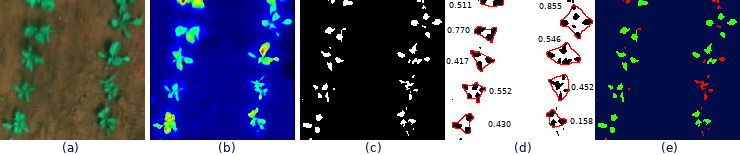
\includegraphics[width=\linewidth]{img/features/pipeline-sub}
        \caption{key steps of image analysis for crop/weed discrimination with (a) acquisition enhancement (b) vegetation indices (c) instance segmentation (d) feature extraction (e) classification}
        \label{fig:pipeline-sub}
    \end{figure}
    
	Major reviews of weed mapping techniques have been carried out by \cite{Monteiro2019}, \cite{GAO201843}, \cite{mostajer2019plant} and \cite{WANG2019226} and show multiple approaches to weed mapping and feature extraction. For example, during the extraction stage, the criteria can be classified according to the nature of the information. We can distinguish (i) shape criteria which are based on different representations of the contours, \cite{AHMED201298, PEREZ2000197}, (2) spatial criteria based on the distance of the individual to another element of the image, such as the distance to the nearest crop row \cite{rs10050761}, (3) texture features based on the analysis of the spatial distribution of the pixels (may include the soil) \cite{Rojas2017} and, finally (4) spectral indices at specific points on the surface can also be used \cite{Liu2019}, which could also be considered as a subset of texture features. However, each type of criterion has different effectiveness and limitations. Spectral and texture features are more affected by illumination variations, while shape features are affected segmentation quality. Moreover, because of these limitations, studies usually combine these types of features to take advantage of all the benefits.
    
    % Shape, position, texture and spectrum analyses offer complementary properties with divergent, and therefore complementary, limits.
    
    However, although these criteria seem to be efficient, they may loose effectiveness in real conditions because they are limited by the previous stages of the pipeline like in Figure \ref{fig:pipeline-sub}. In particular by the plant instance segmentation step, which is still a scientific challenge despite the advances in deep-learning. In this context, we have proposed in a previous study to detect not the whole plant but the leaves which gives promising results in terms of instance segmentation and allows to work in dense foliage \cite{vayssade2022}. Moreover, the leaf offers more stable criteria: there is less intra-individual variability than with a plant. For example, depending on the growth stage, the plant will contain a variable number of leaves with different orientations and sizes, these leaves may also have a partial overlap between them leading to an infinite number of cases. Thus the extracted criteria are viable for a given stage of development, for given crops and specific acquisition conditions.
    
    We will see that some of these issues do not occur at the leaf level. The extracted criteria are also more understandable at leaf scale : shape criterion, such as length or perimeter is less subject to interpretation on the leaf level than on the plant level. Texture criterion, such as gradients, gives the veins of the leaf, but there's no obvious correspondence at the plant scale. Thus the study of these criteria at the leaf scale could be promising to discriminate leaves between crops and weeds. In addition, such leaf-scale criteria have been used successfully for tree species discrimination, \cite{Cerutti2013, Cerutti2014} showing an accuracy up to $90\%$ with only shape criteria at leaf scale for species classification.
    
    Therefore, this study focuses on two points, evaluating criteria that could be used at the leaf level and determining the best criteria combination to discriminate leaves between crops and weeds in field condition. Through this study, we also propose a Python framework allowing the extraction of these criteria available at \url{github.com}.
    
    %Leaf morphological and anatomical traits have been used to discriminate between crop and weed leaves in the past. However, no study has been conducted to determine the best combination of criteria to use in discriminating between crop and weed leaves in field condition. The objectives of this study were to: (1) evaluate criteria that could be used at the leaf level to discriminate between crop and weed leaves in field condition; and (2) determine the best combination of criteria to use in discriminating between crop and weed leaves in field condition.
    %In order to evaluate criteria that could be used at the leaf level to discriminate between crop and weed leaves in field condition, a literature review was conducted. The following criteria were evaluated: leaf shape, leaf size, leaf margin, leaf venation, and leaf color.
    
    %The results of the literature review indicated that leaf shape, leaf size, and leaf margin were the most commonly used criteria to discriminate between crop and weed leaves. However, the results of the study also indicated that there is no consensus on which of these criteria are the best for discriminating between crop and weed leaves.
    
    %In order to determine the best combination of criteria to use in discriminating between crop and weed leaves in field condition, a field experiment was conducted. The experiment was conducted at the Weed Science Research Unit of the University of Saskatchewan. The study site was a mixed cropping system with a two-year rotation of canola, wheat, and flax. The crops were at the vegetative stage (4-6 leaves) and the
    
    \section{Material and data}
    
    \subsection{Experimental plot}
    
    Data is acquired at the site of INRAE in Montoldre (Allier, France, at 46°20'30.3”N 3°26'03.6”E) within the framework of the ANR Challenge RoSE in 2019, visible on Figure \ref{fig:parcelle-xp}. The objective of the Challenge is to objectively compare the solutions proposed by participants \cite{ChallengeRoSE, ChallengeRoSE2021}. Within this context, the challenge provides an evaluation plan to contestants and a set of experimental plots of bean and corn plants. In addition various natural weeds (yarrows, amaranth, geranium, plantago, ...) and sowed ones (mustards, goosefoots, mayweed and ryegrass) is managed to compare performances.
    
    \begin{figure}[H]
        \centering
        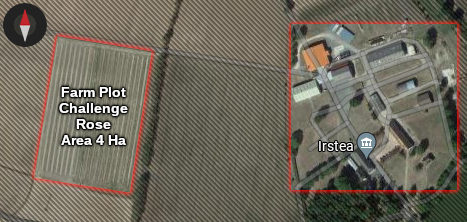
\includegraphics[width=0.5\linewidth]{img/features/parcelle-xp}
        \caption{Aerial view of the experimentation plot located in Montoldre (now INRAE)}
        \label{fig:parcelle-xp}
    \end{figure}
    
    \subsection{Multispectral camera}
    
    The images were acquired with the Airphen (Hyphen, Avignon, France) six-band multispectral camera (Figure \ref{fig:camera-airphen}). This is a multispectral scientific camera developed by agronomists for agricultural applications. The camera has been configured using the 450/570/675/710/730/850 nm bands with a 10 nm FWHM. The focal length of each lens is 8 mm. The raw resolutions for each spectral band are 1280x960 px with 12 bit precision. Due to the conception of the camera, spectral images are not aligned in space. A registration method based on previous work for this camera ,with a registration accuracy down to sub-pixel is used \cite{vayssade:hal-02499730}. After the registration, all spectral bands are rescaled to $1200 \times \SI{800}{px}$ and concatenated to channel-wise where each dimension refers to a spectral band.
    
    \begin{figure}[H]
        \centering
        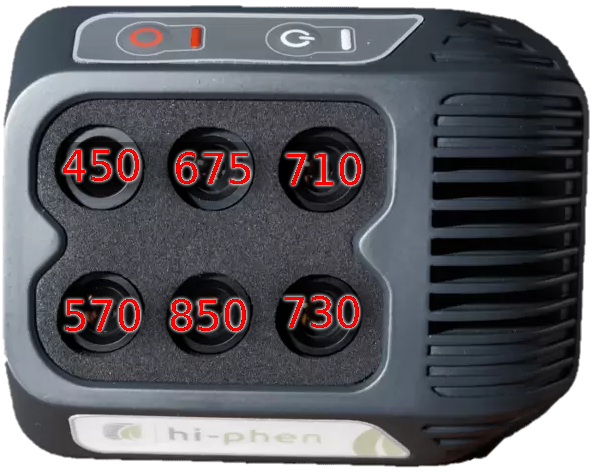
\includegraphics[height=8em]{img/features/camera-airphen}
        \caption{The Airphen six-band multispectral camera}
        \label{fig:camera-airphen}
    \end{figure}
    
    
    \subsection{Image acquisition and annotation}
    
    From the presented experimental plots a set of images were acquired. The camera is attached in front of an hybrid autonomous tractor called ``\textit{TREKTOR}'' launched by \textit{SITIA} (Bouguenais, France) in 2019. The camera is setup to have a top-down view of crop rows, thus it is placed at the end of a 2 m pole in front of the platform allowing to remove visible part of the robot and at 1.8 m from the ground to see all three crop rows. Crops and weeds were between phenological state 3 and 4 which means they had between 2 and 6 leaves. The ground truth is manually defined on images by experts with polygons around each leaf boundaries. In addition, polygons contain a crop/weed classification label. These annotation are performed using the VIA annotation software \cite{dutta2019vgg} and a total of 300 images of bean were annotated, 170 in June and 130 in October. This dataset is now available online\footnote{\url{https://data.inrae.fr/dataset.xhtml?persistentId=doi:10.15454/JMKP9S&version=1.0}} and may help other studies working on leaves classification. In addition the crop rows for each image are also manually set. The total number of leaves is \SI{90538}, with \SI{31524} for crops and \SI{59019} for weeds.
    
    \section{Methodology}
    
    The objective of this paper is to extract a wide variety of features and evaluate their performances for classifying leaves into crops and weeds, in addition to defining the best subset of feature space. The methodology followed in this study is as follows:
    
    \begin{enumerate}
        \item In order to evaluate criteria that could be used at the leaf level to discriminate between crop and weed leaves in field condition, a literature review was conducted. These criteria are organized into shape, spatial and textural features and presented in the section \ref{sec:weed-discrimination-extracted-features}.
        
        \item Most of the features have parameters that impact the extraction and classification performances of these features. To solve this problem, we propose to optimize these parameters by using an hyperparameter optimisation algorithm to efficiently sample the parameter space, it is described in section \ref{sec:weed-discrimination-optimization}.
        
        \item The results of the literature review indicate that there is no consensus on which of these criteria are the best for discriminating between crop and weed (at plant or leaf scale). In order to determine the best combination of criteria to use in discriminating between crop and weed leaves in field condition, an algorithm to select the best subsets of features is used and described in section \ref{sec:weed-discrimination-fv-selection}.
        
        \item The performance of each method is evaluated on the ground truth dataset, using Area Under the Curve (AUC) as the performance metric. The best performing feature subset is presented to classify leaves into crops and weed. These subsets are extracted for each type of feature (locally) and among all feature (globally), this is available in the results section \ref{sec:weed-discrimination-results}.
        
        \item Finally a classification of the vegetation cover is proposed using the best performing features subsets and the results are discussed in section \ref{sec:weed-discrimination-best-all}.
    \end{enumerate}
    
    %These features are based on spatial, texture or shape information, and are described in the next subsection \ref{sec:weed-discrimination-extracted-features}. On the other hand in this paper, we do not evaluate the effect of the segmentation procedure. Thus, the features are directly extracted from the ground truth.
    
    %%%%%%%%%%%%%%%%%%%%%%%%%%%%%%%%%%%%%%%%%%%%%%%%%%%%%%%%%%%%%%%%%%%%%%%%%%%%%%%%%%%%%%%%%%%%%%%%
    
    \subsection{Literature review}
    \label{sec:weed-discrimination-extracted-features}
    
    In computer vision, shape, spatial and textural features are commonly used for describing and classifying objects. In this section we will present a review of these features. To facilitate the extraction of features and their merging, they have been programmed using the OOP \footnote{Object-Oriented Programming} paradigm in Python. Each feature is thus named according to its type (shape / spatial / spectral) and internal properties. Thus the following subsections present each of them according to its type.
    
    \subsubsection{Shape Criteria}
    
    Shape properties are based on a structural analysis of the contours of related regions, it mostly consists of detecting morphological and anatomical traits.	The shape can be coded as a set of positions (pixels) that go around the boundary. From this description, various information can be used. This type of analysis is found particularly in granulometry \cite{hentschel2003selection}, geomatics \cite{mcgarigal1995spatial}, leaf classification \cite{Cerutti2014} or even animal posture detection \cite{vayssade2019automatic, Bonneau2021}. These criterion are the most intuitive, easy to implement, and unaffected by lighting. Each of the following paragraphs explain an extraction method as well as the resulting properties used for discrimination.
    
    \newpage
    \paragraph{Shape Ellipse} \cite{watcharabutsarakham2012leaf} have mentioned that the major and minor axis can be used to classify leaves. These properties can be obtained through an elliptical Hough algorithm as described by the article. From the retrieved ellipse, few more information can be compute such as the distance between the ellipse center and the detected shape center. Three factors of eccentricity, the directrix, the angle and the focal distance. Some of these properties were also used by \cite{Lottes2016} for the classification of plant covers.
    
    \paragraph{Shape Particle} Based on the work of \cite{hentschel2003selection}, these shape metrics have been used to characterise and classify particles. \cite{vayssade2019automatic} used it to classify goats activities within pasture, \cite{Bonneau2021} to estimate the sow posture with an accuracy near deep-learning methods (\SI{94}{\percent} vs \SI{96}{\percent}). This set of 18 characteristics are based on a variety of ratios of the Feret diameter, area and perimeter. Some of them are known as : Equivalent Diameter, Eccentricity, Aspect Ratio, Form Factor, Roundness or Convexity. Others are unnamed features. The Feret diameter is defined as (1) the longest distance between two points on the contour, and (2) the shortest distance across the shape. Some of these properties are also used by \cite{Lottes2016} and \cite{saha2017development}.
    
    \paragraph{Shape Solidity} The solidity factor is widely used for weed plant classification \cite{AHMED201298}. The solidity factor is defined as a ratio between the segmentation mask area and convex hull area. Thus, it is bound from 0 to 1. This factor indirectly computes the holes area of the regions. When applied to weed discrimination, this factor allows to discriminate some specific species like carrot from others. When carrots are segmented, the segmentation mask is sparse, filled by a large amount of holes, due to leaves structures. This does not occur for dicotyledon plants, and it is less impacted by other monocotyledons weeds. At leaf scale, such criteria provide information about the contour (leaf teeth) as the inner leaf mask should be filled. This approach has been used for species classification \cite{thyagharajan2019review} and weed discrimination \cite{Lottes2016}. 
    
    \paragraph{Shape Metrics} This set of 8 properties comes from the documentation of the shape metrics tools of the University of Connecticut \footnote{\url{http://clear.uconn.edu/tools/Shape_Metrics/method.htm}}, these are used for shape classification of lands \cite{angel2010ten} and building \cite{paszto2015shape}. Few properties, such as Cohesion, Traversal, Range and Viable Interior was not implemented due to time complexity. The others 8 implemented metrics are named : Proximity, Exchange, Spin, Perimeter Index, Depth, Girth, Dispersion and Detour.
    %!TODO revenir dessus -> temps de calcule
    %set de 12 pptés, 8 utilisées
    %Range
    
    \paragraph{Shape Fragstat} The book by \cite{mcgarigal1995spatial} shows some of the features used at the landscape, class, or parcel scale for classification or shape similarity measures. The fragstats documentation shows a small set of criteria \footnote{\url{http://www.umass.edu/landeco/research/fragstats/documents/Metrics/Shape\%20Metrics/SHAPE\%20METRICS.htm}} that can be exploited at the leaf scale such as: Perimeter-Area Ratio, Shape Index, Fractal Dimension Index, Linearity Index, Related Circumscribing Circle, Contiguity Index and the Perimeter Area Fractal Dimension. These features have been selected as shape criterion in our study because they reflects shape complexity for a given spatial scale and correspond to: Perimeter-area-ratio, Shape Index, Fractal Dimension Index, Linearity Index, Related Circumscribing Circle, Contiguity Index and Perimeter Area Fractal Dimension.
    %  Only individual properties are exploited (at entity level), the normalization of some properties (4) are not implemented to reduce complexity.
    
    \paragraph{Shape Skeletonize} The skeletonization is commonly used in shape recognition techniques. It transforms the input mask (i.e the shape) to a new structural representation of the shape \cite{ERDEM20102024}. This representation captures part of internal hierarchy. As instance, the \cite{Lottes2016} study use the skeleton length for weed discrimination. In this study more features are extracted from that structural representation. These properties are defined as : the number of $end\_ point$, the number of internal $branches$, the number of $intersections$ and the total length of the skeleton ($pixel\_count$).
    
    \paragraph{Shape Angle} The distribution of angles between points around the contours can be exploited to measure the similarities between shapes \cite{belongie2002shape}. This method was used to classify symbols (digits and letters). The procedure is defined as follow: for a point of the contour, we compute the relative angles of all the other points that are in a given radius. The radii and angles are stored in a ``shape matrix'' of dimensions: $radial\_bins \times angle\_bins$. Each element $(i,j)$ of the matrix contains a counter which corresponds, for a given point, to the number of points which are in this bin of radius $i$ and in the bin of angle $j$. Finally, the procedure is repeated for each point of the contour to feed the ``shape matrix''. This one is used as a discriminating variable.
    %https://www2.eecs.berkeley.edu/Research/Projects/CS/vision/shape/belongie-pami02.pdfs
    
    \paragraph{Shape Hu Moments} The Hu Moments have been proposed long time ago by \cite{hu1962visual} and are part of structural analysis. The contours of the related regions are transformed into ``moments'', which are then transformed into Hu Moments. The importance of this extraction comes from its translation, rotation, and scaling invariance. A similar element, e.g. two different bean leaves at various positions, rotation or scale will then be represented identically. This assertion remains true if intra-species and intra-individual variability are not taken into account. Hu Moment have been used for leaf classification challenge \cite{rhouma2017moment}.
    
    %%%%%%%%%%%%%%%%%%%%%%%%%%%%%%%%%%%%%%%%%%%%%%%%%%%%%%%%%%%%%%%%%%%%%%%%%%%%%%%%%%%%%%%%%%%%%%%%
    
    \subsubsection{Spatial Criteria}
    
    The spatial properties are based on the extraction of global information related to the agricultural plot. These extraction methods are based on a distance which is calculated between the extracted global information and the centroid of the related region. The distribution of the values is strongly correlated to the vegetation density, allowing to discriminate the weeds, mostly between rows.
    
    \paragraph{Spatial Row} The distance between the plant and the crop line is one of the most used spatial descriptors when such prior knowledge is observable \cite{rs10050761, Koot891024465110, DBLP:journals/corr/abs-1805-12395}. The number of techniques to extract such rows within an agronomic images is large, most of them are based on Hough Transform applied to line detection, as \cite{rs10050761}. Recent studies in deep-learning shows that CNN can be used to detect crop row in agricultural acquisition \cite{bah2019crownet}. As the objective of this section is to evaluate the impact of the distance between plants and crop row (not the row detection performance), this study uses the crop rows from the ground truth.
    
    % unreleavant properties 51.76%
    \newpage
    \paragraph{Spatial Blob} In most cases, plants can be classified into two types: monocotyledons and dicotyledons. At an early stage, when the plant emerges from the ground, its appearance is totally different according to this initial type. Monocotyledons usually looks like a filament, while dicotyledons look like an oval shape when seen from above. With this information, a specific shape detection algorithm can be implemented. Such as Blob detection, which aims to detect groups of connected pixels in an image that share a common property (shape, color, \dots). The objective of Blob detection is to identify and mark these regions. These marks are used to calculate the Euclidean distance between the centroid of leaf and the nearest blob. Thus, the distribution of values is strongly correlated to the density of vegetation. This is an hypothesis we want to test and we have not seen any article using this type of approach.
    
    % unrelevant properties 56.59%
    \paragraph{Spatial Corner} The detection of points of interest can be used to discriminate weeds. This is what is proposed in the article of \cite{agronomy10010113}, using an algorithm of detection of corners in the image. From these points of interest, the distance and the angle between the center of the plant and the closest points of interest are used as discriminating properties. In reality, this detection finds the leaves apexes. Here only the distance between the centroid and the nearest points of interest is computed since the angle is already present in Shape Ellipse properties.
    
    %%%%%%%%%%%%%%%%%%%%%%%%%%%%%%%%%%%%%%%%%%%%%%%%%%%%%%%%%%%%%%%%%%%%%%%%%%%%%%%%%%%%%%%%%%%%%%%%
    
    \subsubsection{Textural, Color and Spectral Criteria}
    
    Texture properties are vast and include many things, like image transformations (Fourier, Wavelets, color spaces, \dots), color, spectral properties or histograms to characterise observed surfaces. The article \cite{mekhalfa2021supervised}, have tested texture and color properties on RGB images of soybeans. The proposed color characteristics, are the means and standard deviations of the image in two color spaces (RGB and HSV). In terms of texture properties, i.e. an analysis of the spatial distributions of the colors, the paper relies on GLCM (Gray-Level Cooccurrence Matrix), Haralick and LBP (Local Binary Pattern) features. According to the study, the results are based on these properties and gave classification rates between \SI{89.43}{\percent} and \SI{96.17}{\percent}. Here, we have extended this work by adding their location to the extracted properties. %extending both the properties and the location where they are extracted%
    Thus, all the extractions defined hereafter are automatically done on each individual bands, on NDVI and on the standard deviation (std) between spectral bands (which is also an image).
    
    \paragraph{Spectral Signature} The spectral signature is defined as the value (at the center of the shape and at the center of its bounding box) of all spectral bands, the NDVI value and the standard deviation between spectral bands.
    
    \paragraph{Spectral Stats} As shown by \cite{Lottes2016}, statistical properties of the underlying bounding box (that contains the shape) can be computed and used for weed discrimination. According to this article, a set of nine properties for each spectral bands is extracted separately as well as a vegetation index (NDVI) and the standard deviation (std). These properties are based on color moments (Table \ref{tab:colors-moments}).
    
    \vfill
    \begin{table}[H]
        \centering
        \rowcolors{0}{gray!10}{white}
        \begin{tabular}{c c c}
            \hline
            min & max & range \\
            mean & std & median \\
            skewness & kurtosis & entropy \\
            \hline
        \end{tabular}
        \caption{Synthesis of colors moments}
        \label{tab:colors-moments}
    \end{table}
    \vfill
    
    \newpage
    \paragraph{Spectral HoG} The HoG descriptors for Histogram of Oriented Gradient was used by \cite{saha2017development} for weed discrimination. It is often used in computer vision, both for object detection and texture discrimination because of its properties of geometric invariance. The HoG descriptors are based on gradient intensity and edge directions. From this information, a histogram is computed and used as descriptor. Applied to a leaf, theses properties allow to characterise leaf veins \cite{tsolakidis2014plant}. This features are generally robust to illumination changes and color differences due to the leaf maturity.
    
    \paragraph{Spectral Hu Moment} Moments and Hu Moments are generally applied to segmentation masks or contours. It retrieves shape properties, such as perimeter, centroid, etc. Computing these features on spectral bands and NDVI could include more discriminating information. This is an assumption that we wish to verify and there is no anterior of such use.
    
    % not releavant feature -> 50% of classification score
    %\paragraph{Spectral DoG} The Difference of Gaussian, \cite{Munzenmayer:2002:MTA:648287.754097}
    % https://link.springer.com/chapter/10.1007/3-540-45783-6_6
    
    \paragraph{Spectral Gabor} Gabor filters have been widely used for texture analysis in mono-bands images. By extension, \cite{650858} have proposed to use properties based on the results of Gabor filters applied to multispectral texture classification. They use a set of symmetric and circular Gabor filters, with three octave scales and four orientations to compute properties, such as averages and energy. These filters have been used in the field of weed discrimination by \cite{Ishak2009}. In the current study, a symmetric and circular Gabor filters are applied with a single (optimized) octave scale and four orientations ($[0,40,90,158]$) as defined by \cite{650858}. However, extracted properties from such filters are based on color moments (Table \ref{tab:colors-moments}) on each Gabor orientation filter.
    
    \paragraph{Spectral LBP} The LBP descriptor, for Local Binary Pattern is a feature that encodes texture information. The general principle of LBP is to compare the level of a pixel luminance with the levels of its neighbours (0 if inferior, and 1 else). Depending on the neighbour position, a weight is applied to the positive value ($[1,2,4,8,16,32,64,128]$), the LBP value is then the sum of weighted positives values. The last feature, is the histogram of the leaf texture for each spectral bands and NDVI. This gives an account of information relating to regular patterns in the image, in other words texture.
    
    \paragraph{Spectral CSLBP} The CS-LBP operator for Center-Symetric Local Binary Pattern is an extension of the previously defined LBP operator \cite{Banerji2003Chapter1L}. For each pixel, the absolute and symmetric difference of the neighborhood is computed, if the value is higher than a fixed threshold $T=0.1$ the element takes the value $1$ ($0$ otherwise). The set of results is coded as LBP through a weighted sum depending on the neighbour location. These features are considered to be more robust against rotation than standard LBP. This is an assumption that we wish to verify.
    
    \paragraph{Spectral OCLBP} The OC-LBP (Opposite Color LBP) operator is an extension of the LBP operation. \cite{Banerji2003Chapter1L} propose an LBP extension to the colorimetric domain by considering the inter channel relationship instead of local and spatial relationship of a pixel. For each color pair $(u,v), u>v$ the inter-channel properties are considered by $C=I(x,y,u) - I(x,y,v))$. With $I$ the multispectral image, $x,y$ the pixel position and $u,v$ the color channels to compare. The obtained image is defined in the same way as LBP: a weighted sum of positives values. These properties have been used by \cite{7566749} for grape plant diseases detection.% and decision support.%
    
    \paragraph{Spectral GLCM} This is a square matrix of dimension $N_g$, where $N_g$ is the number of gray levels in the image. The $[i,j]$ element of the matrix is generated by counting the number of times a pixel of value i is adjacent to a pixel of value j, and then dividing the entire matrix by the total number of comparisons made. Each entry is thus considered as the probability that a pixel of value i is adjacent to a pixel of value j denoted $p(i,j)$, defining for us the co-occurrence matrix $G$. This have been used by \cite{bakhshipour2017weed} for weed discrimination.
    
    \paragraph{Spectral Haralick} The basis of these features is the GLCM (grayscale co-occurrence matrix). From that, Haralick have defined 14 texture descriptors that can be computed. This estimator was tested for canopy discrimination by \cite{wong2013co}.
    
    \paragraph{Spectral Polyfit} We introduce a new type of feature based on polynomial fitting. Multispectral images may lack information due to the selection of the spectral domain (The Airphen camera uses 6 spectral bands). To recover the original spectrum distribution across the surface, a simple solution that can be used is curve fitting \cite{1634723}, by using the value of observed pixel and their distances to the center of the shape. The result of the fitting is the polynomial parameter, which can be used as a discriminant variable.
    
    
    \paragraph{Spectral Shi Tomasi} The Shi-Tomasi feather is a kind of key point detector using the eigenvalue of the second moment of the color matrix \cite{harris1988combined}. On these values, a threshold is applied to determine if a pixel can be a corner or not. This algorithm has an interesting step, it transforms the input color image space into a gray scale color space, through this eigenvalue decomposition. Here, instead of finding the local maxima of this transformation, which are the key points. We propose to use a small histogram to describe the observed surface, so the values of corresponding to a corner accumulate in a specific bins of the histogram, while flat surfaces accumulate on other bins, etc. This transformation is applied on the first 3 bands of our data (450 nm, 570 nm, 650 nm) which are nearest to a RGB color space.
    
    %L'indice de végétation (RGB) peut être interprété comme étant une information 3D (Gradient + Magnitude),
    %L'indice est transformé en calculant la nouvelle image par $sensitivity * \sqrt{(B-G)^2 + 4 + (2R-1)^2}$.
    %Un histogramme est ensuite estimé pour les valeurs internes à la forme détectée.
    
    %%%%%%%%%%%%%%%%%%%%%%%%%%%%%%%%%%%%%%%%%%%%%%%%%%%%%%%%%%%%%%%%%%%%%%%%%%%%%%%%%%%%%%%%%%%%%%%%
    
    \subsection{Optimization}
    \label{sec:weed-discrimination-optimization}
    
    Some features have parameters, like the number of bins in case of histogram analysis, the $inner$ and $outer$ radius of ``shape angles'' and so on. Some parameters are discrete numbers, but others are in a continuous space, like four parameter of the ``texture gabor'' which requires to set them before using it (sigma, lm, gm, ps). Setting these parameters has a critical impact on classification performances, they can be set empirically. But to optimize the performances of extracted features, these parameters must be optimized properly and automatically. This is known as an hyperparameter optimization problem.
    
    There are many ways to sample the parameter space. One approach is grid search, where the parameter space is divided into a number of discrete regions (or grids) and a search is performed in each point of the grid \cite{lawler1966branch}. Another approach is random search, where a random point is chosen in the parameter space and the performance if evaluated \cite{bergstra2012random}. However, they can also lead to suboptimal solutions, because both methods are brute force approaches that scale poorly with the hyperparameters number. Therefore, it is important to choose an appropriate sampling method for the problem at hand. To achieve this optimization, more complex algorithms must be used to sample the parameter space efficiently.
    
    \newpage
    We propose to use an asynchronous early stop method based on the continuous halving algorithm to solve this challenge, this is the ASHA algorithm (Asynchronous Successive HAlving). The ASHA algorithm is a randomized, asynchronous and incremental algorithm for sampling the parameter space. It is based on the continuous halving algorithm, which is a greedy algorithm that divides the parameter space into two halves and selects the best half at each step. The ASHA algorithm uses this approach to iteratively divide the parameter space into smaller subsets. At each step, it selects the best subset based on a performance metric and stops when the subset is small enough that the performance is no longer improving. This approach is more efficient than grid search or random search, because it can find good solutions without exploring the entire parameter space. The asynchronous part of this algorithm allows it to run on multiple processors, which can speed up the search \cite{hertel2020sherpa}.
    
    In addition, to sample the parameter space correctly, each parameter has been manually bounded to limit the search space. The ASHA algorithm has been implemented in the Sherpa software package \cite{hertel2020sherpa} in Python. Finally, the optimization is done through \SI{10000} epochs. At each epoch a 2-fold cross-validation is used for training and validating a decision tree classifier. This should enforce the learning of more stable properties and avoid overfitting, because the first fold contains the majority of data obtained in June, while the second fold contain the data obtained in October. The decision tree classifier is chosen to use simple decision criteria, rather than complex model, to extract most relevant features. The performance of the extracted features is therefore the performance of the underlying learned classifier (average of the cross-validation procedure). The Figure \ref{fig:hp-optimization} synthesizes the optimization procedure :
    
    %, so the best parameters found are those that lead to the lowest validation error on the cross-validation set.
    
    \vfill
    \begin{figure}[H]
        \centering
        \vspace{-2em}
        \tikzset{
	ppblock/.style={
		rectangle,
		minimum size=6mm,
		very thick,
		draw=black!50,
		text centered,
		font=\ttfamily,
		minimum width=8em,
		minimum height=6mm,
		top color=white,
	},
	%
	figure/.style={
		rectangle,
		rectangle split,
		rectangle split parts=2,
		very thick,
		draw=black!50,
		text centered,
		append after command={
			\pgfextra
			\fill[top color=#1, bottom color=#1]
			(\tikzlastnode.one west) 
			[rounded corners] |- (\tikzlastnode.north) -| (\tikzlastnode.one east) 
			[sharp corners]   |- (\tikzlastnode.one split) -| cycle;
			\fill[top color=white, bottom color=#1]
			(\tikzlastnode.two west) 
			[rounded corners] |- (\tikzlastnode.south) -| (\tikzlastnode.two east)  
			[sharp corners]   |- (\tikzlastnode.one split) -| cycle;
			\endpgfextra
		},
	},
    splitted/.style={
        rectangle,
        rectangle split,
        rectangle split horizontal,
        rectangle split parts=2,
        very thick,
        draw=black!50,
        text centered,
        append after command={
            \pgfextra
            \fill[top color=white, bottom color=#1]
            (\tikzlastnode.south)
            [rounded corners] -| (\tikzlastnode.west) |- (\tikzlastnode.one north)
            [sharp corners]   -| (\tikzlastnode.one split) |- cycle;
            \fill[top color=white, bottom color=#1]
            (\tikzlastnode.two south)
            [rounded corners] -| (\tikzlastnode.east) |- (\tikzlastnode.north)
            [sharp corners]   -| (\tikzlastnode.one split) |- cycle;
            \endpgfextra
        },
    },
	%
	static/.style={ppblock, bottom color={black!20}},
	nonterminal/.style={ppblock, bottom color={blue!30}},
	terminal/.style={ppblock, bottom color={green!20}},
	algorithm/.style={ppblock, bottom color={yellow!50}},
	error/.style={ppblock, bottom color={red!20}},
	type/.style={ppblock, bottom color={red!20}},
	loss/.style={ppblock, dashed, bottom color={black!20}, font=\itshape},
	%
	tiny/.style={
		rounded rectangle,
		very thick,
		draw=black!50,
		top color=white,
		bottom color=red!20,
        text centered,
		font=\ttfamily,
	},
    operator/.style = {
        circle,
        scale=0.6,
        draw=black!50,
        top color=white,
        bottom color=red!20,
        font=\boldmath,
    },
	%
	skip loop/.style={to path={-- ++(0,#1) -| (\tikztotarget)}}
}
%\vspace{-3em}
\begin{tikzpicture}[
    >=stealth',thick,
    tip/.style={->,shorten >=0.007pt},
    every node/.style={scale=0.8},
]
\matrix[column sep=8mm, row sep=4mm, align=center] {
	\node (hp)     [nonterminal]   {Hyper\\Parameters};         &
	\node (oa)     [algorithm]     {Optimization\\Algorithm};           &
	\node (bm)     [terminal]      {Best Model};               \\
	
	
	\node (fv)     [nonterminal]   {Feature\\Extraction};         &
	\node (oj)     [loss]          {Objective};         \\
	
	\node (ds)     [type]     {Dataset};         &
	\node (cv)     [static]   {Cross-Validation};         &
	\node (dt)     [static]   {DecisionTree};         &
	\\
};

\draw[->] (hp) to (fv);
\draw[->] (fv.south east) to (cv.north west);
%\draw[->] (ds) to (cv);
\draw[->] (ds) to (fv);
\draw[->] (dt) to (cv);
\draw[->] (cv) to (oj);
\draw[->] (oj) to (oa);
\draw[->] (oa) to (hp);
\draw[->] (oa) to (bm);
\end{tikzpicture}
        \caption{Hyperparameter optimization procedure}
        \label{fig:hp-optimization}
    \end{figure}
    \vfill
    
    %\begin{figure}[H]
    %    \centering
    %    \tikzset{
	ppblock/.style={
		rectangle,
		minimum size=6mm,
		very thick,
		draw=black!50,
		text centered,
		font=\ttfamily,
		minimum width=8em,
		minimum height=6mm,
		top color=white,
	},
	%
	figure/.style={
		rectangle,
		rectangle split,
		rectangle split parts=2,
		very thick,
		draw=black!50,
		text centered,
		append after command={
			\pgfextra
			\fill[top color=#1, bottom color=#1]
			(\tikzlastnode.one west) 
			[rounded corners] |- (\tikzlastnode.north) -| (\tikzlastnode.one east) 
			[sharp corners]   |- (\tikzlastnode.one split) -| cycle;
			\fill[top color=white, bottom color=#1]
			(\tikzlastnode.two west) 
			[rounded corners] |- (\tikzlastnode.south) -| (\tikzlastnode.two east)  
			[sharp corners]   |- (\tikzlastnode.one split) -| cycle;
			\endpgfextra
		},
	},
    splitted/.style={
        rectangle,
        rectangle split,
        rectangle split horizontal,
        rectangle split parts=2,
        very thick,
        draw=black!50,
        text centered,
        append after command={
            \pgfextra
            \fill[top color=white, bottom color=#1]
            (\tikzlastnode.south)
            [rounded corners] -| (\tikzlastnode.west) |- (\tikzlastnode.one north)
            [sharp corners]   -| (\tikzlastnode.one split) |- cycle;
            \fill[top color=white, bottom color=#1]
            (\tikzlastnode.two south)
            [rounded corners] -| (\tikzlastnode.east) |- (\tikzlastnode.north)
            [sharp corners]   -| (\tikzlastnode.one split) |- cycle;
            \endpgfextra
        },
    },
	%
	static/.style={ppblock, bottom color={black!20}},
	nonterminal/.style={ppblock, bottom color={blue!30}},
	terminal/.style={ppblock, bottom color={green!20}},
	algorithm/.style={ppblock, bottom color={yellow!50}},
	error/.style={ppblock, bottom color={red!20}},
	type/.style={ppblock, bottom color={red!20}},
	loss/.style={ppblock, dashed, bottom color={black!20}, font=\itshape},
	%
	tiny/.style={
		rounded rectangle,
		very thick,
		draw=black!50,
		top color=white,
		bottom color=red!20,
        text centered,
		font=\ttfamily,
	},
    operator/.style = {
        circle,
        scale=0.6,
        draw=black!50,
        top color=white,
        bottom color=red!20,
        font=\boldmath,
    },
	%
	skip loop/.style={to path={-- ++(0,#1) -| (\tikztotarget)}}
}
\begin{tikzpicture}
    \matrix (M) [
        matrix of nodes,
        nodes={
            minimum height = 6mm,
            minimum width = 1.5cm,
            outer sep=0,
            anchor=center,
            draw,
            scale=0.9
        },
        column 1/.style={nodes={draw=none}, minimum width = 4cm},
        column 4/.style={nodes={draw=none}, minimum width = 1cm},
        row sep=1pt, column sep=-\pgflinewidth, nodes in empty cells,
        t/.style={minimum width = 3.75cm, top color=white, bottom color=green!20},
        e/.style={minimum width = 3.75cm, top color=white, bottom color=red!20},
    ]
    {
        Fold 1 & |[t]| train & |[e]| test  & $AUC_1$ \\
        Fold 2 & |[e]| test  & |[t]| train & $AUC_2$ \\
    };
    
    \draw (M-1-2.north west) ++(0,2mm) coordinate (LT) edge[|<->|, >= latex] node[above,scale=0.7]{Total number of images} (LT-|M-1-3.north east);
    
    \draw[decoration={brace,raise=-7pt,amplitude=4pt},decorate,line width=1pt] 
    ([yshift=-5pt]M.north east) -- ([yshift=5pt]M.south east);
    
    \node  at (6.1,0) {$\frac{1}{2} \sum_{i=1}^{2}{AUC_i}$};
\end{tikzpicture}
    %    \vspace{-1em}
    %    \caption{The 2-fold cross-validation procedure}
    %    \label{fig:cross-validation-2}
    %\end{figure}
    
    As an example, Table \ref{tab:asha}, show 5 epochs for the optimization of spectral Gabor features (parameters: sigma, lm, gm and ps), the objective value is the value to be maximized, it corresponds to the performances of classification model evaluated by the \textit{Area Under the Curve} metric \cite{FAWCETT2006861}. % After the optimization, the number of feature can be see in Table \ref{tab:optimized_features} in appendix.
    After the optimization process, all features are extracted.
    
    \vfill
    \begin{table}[H]
        \centering
        \rowcolors{0}{gray!10}{white}
        \begin{tabular}{|c|cccc|c|} \hline
            \textbf{Epoch} & \textbf{sigma} & \textbf{lm} & \textbf{gm} & \textbf{ps} & \textbf{Objective} \\ \hline
            1616 & 1.865 & 5.720 & 0.409 & 0.403 & \cellcolor{green!25}{0.621} \\
            1617 & 1.838 & 5.732 & 0.363 & 0.421 & 0.604 \\
            1618 & 1.894 & 4.960 & 0.431 & 0.335 & 0.556 \\
            1619 & 3.363 & 8.253 & 0.083 & 0.690 & 0.465 \\
            1620 & 7.705 & 4.655 & 0.986 & 0.090 & 0.517 \\ \hline
        \end{tabular}
        \caption{Five epochs of the optimization procedure through ASHA algorithm. The objective column show the model performance}
        \label{tab:asha}
    \end{table}
    \vfill \null
    
    \newpage
    \subsection{Feature Selection}
    \label{sec:weed-discrimination-fv-selection}
    
    Now that all the features are optimized and extracted, the main question of this article can be explored. What are the best features to classify leaves into crops and weeds. Since the number of features is huge (\SI{3545}), as shown in Table \ref{tab:optimized_features}, a manual estimation of each feature performances cannot be established properly. To answer this question, researchers in this field typically use a metric to estimate how well a feature fits the problem (correlation coefficient or root mean squared error), and then the best features are used. However, a better combination might exist, e.g., merging two high rank criteria might be less accurate than merging a high rank with a low rank. As an example, row distance and a texture characteristic, the efficiency may be greater than that of two texture criteria, because row distance is likely complementary to texture property. This i an assumption we wish to verify.
    %, even if this property is not able to discriminate intra-row individuals contrarily to the texture properties. \textcolor{red}{rmq: ref?}
    
    Instead of evaluating each feature through a metric, a data mining technique is proposed, such as ``Sequential Forward Selection'' (SFS) \cite{SFS-574797}. It is an algorithm that analyzes each feature to check whether it is going to be useful for the classification task. To put it in another way the motivation behind this algorithm is to automatically select the subset of features most relevant to the problem. Thus, it reduces the initial $d$-dimensional feature space to a $k$-dimensional feature subspace, where $k<d$. The figure \ref{fig:sequential-feature-selection} shows how the algorithm works :
    
    %\begin{enumerate}
    %    \item Start with an empty feature subspace $X_0=\emptyset$ and $k=0$
    %    \item Build all new features spaces $S_i$ that are the union of one feature $F_i$ and the current feature space $X_k$.
    %    \item For each new features spaces $S_i$ an ExtraTree is learned (\cite{geurts2006extremely}) through a 5-fold cross-validation (like in Figure \ref{fig:cross-validation-5}) which estimates the accuracy of the classification model.
    %    \item Among all the new subsets $S_i$, the new best subset is determined through its underlying classifier score and used as X_{k+1}$.
    %    \item This procedure is repeated until the subfeature space $X_k$ have the right dimensions.
    %\end{enumerate}
    
    \begin{figure}[H]
        \centering
        \tikzset{
	ppblock/.style={
		rectangle,
		minimum size=6mm,
		very thick,
		draw=black!50,
		text centered,
		font=\ttfamily,
		minimum width=8em,
		minimum height=6mm,
		top color=white,
	},
	%
	figure/.style={
		rectangle,
		rectangle split,
		rectangle split parts=2,
		very thick,
		draw=black!50,
		text centered,
		append after command={
			\pgfextra
			\fill[top color=#1, bottom color=#1]
			(\tikzlastnode.one west) 
			[rounded corners] |- (\tikzlastnode.north) -| (\tikzlastnode.one east) 
			[sharp corners]   |- (\tikzlastnode.one split) -| cycle;
			\fill[top color=white, bottom color=#1]
			(\tikzlastnode.two west) 
			[rounded corners] |- (\tikzlastnode.south) -| (\tikzlastnode.two east)  
			[sharp corners]   |- (\tikzlastnode.one split) -| cycle;
			\endpgfextra
		},
	},
    splitted/.style={
        rectangle,
        rectangle split,
        rectangle split horizontal,
        rectangle split parts=2,
        very thick,
        draw=black!50,
        text centered,
        append after command={
            \pgfextra
            \fill[top color=white, bottom color=#1]
            (\tikzlastnode.south)
            [rounded corners] -| (\tikzlastnode.west) |- (\tikzlastnode.one north)
            [sharp corners]   -| (\tikzlastnode.one split) |- cycle;
            \fill[top color=white, bottom color=#1]
            (\tikzlastnode.two south)
            [rounded corners] -| (\tikzlastnode.east) |- (\tikzlastnode.north)
            [sharp corners]   -| (\tikzlastnode.one split) |- cycle;
            \endpgfextra
        },
    },
	%
	static/.style={ppblock, bottom color={black!20}},
	nonterminal/.style={ppblock, bottom color={blue!30}},
	terminal/.style={ppblock, bottom color={green!20}},
	algorithm/.style={ppblock, bottom color={yellow!50}},
	error/.style={ppblock, bottom color={red!20}},
	type/.style={ppblock, bottom color={red!20}},
	loss/.style={ppblock, dashed, bottom color={black!20}, font=\itshape},
	%
	tiny/.style={
		rounded rectangle,
		very thick,
		draw=black!50,
		top color=white,
		bottom color=red!20,
        text centered,
		font=\ttfamily,
	},
    operator/.style = {
        circle,
        scale=0.6,
        draw=black!50,
        top color=white,
        bottom color=red!20,
        font=\boldmath,
    },
	%
	skip loop/.style={to path={-- ++(0,#1) -| (\tikztotarget)}}
}
%\vspace{-3em}
\begin{tikzpicture}[
    >=stealth',thick,
    tip/.style={->,shorten >=0.007pt},
    every node/.style={scale=0.8, minimum width=10em},
]
\matrix[column sep=4mm, row sep=4mm, align=center] {

    & & \node (init)     [splitted={green!20}]   {$X=\emptyset$  \nodepart{second} $k=0$}; &       \\
    
    \coordinate (top-left); & & \node (Xs)     [nonterminal]   {Expand $X$}; &       \\
    %& &       \\
	
	&\node (s0)    [nonterminal]   {$S_0=X \cup F_0$};        &
	\node (si)     [nonterminal]   {$S_i=X \cup F_i$};                   &
	\node (sn)     [nonterminal]   {$S_D=X \cup F_D$};        \\
	
	&\node (c0)    [nonterminal]   {ExtraTree\\Cross-Validation};        &
	\node (ci)     [nonterminal]   {ExtraTree\\Cross-Validation};        &
	\node (cn)     [nonterminal]   {ExtraTree\\Cross-Validation};        \\
	
	&\node (o0)     [loss]   {$Objective=0.51$};        &
	\node (oi)     [loss]   {$Objective=\dots$};       &
	\node (on)     [loss]   {$Objective=0.74$};        \\
	%& &       \\
	
	\coordinate (bottom-left); & & \node (bs)     [nonterminal]   { $X = \texttt{Best}(S_i) $}; &       \\
	& & \node (Xn)     [splitted={green!20}]   {$X=\{F_0 | F_3 | F_8 | \dots\}$  \nodepart{second} $k=K$}; &       \\
};

\draw[->] (init) to (Xs);
\draw[->] (Xs) to (s0);
\draw[->] (Xs) to (si);
\draw[->] (Xs) to (sn);

\draw[->] (s0) to (c0);
\draw[->] (si) to (ci);
\draw[->] (sn) to (cn);

\draw[->] (c0) to (o0);
\draw[->] (ci) to (oi);
\draw[->] (cn) to (on);

\draw[->] (o0) to (bs);
\draw[->] (oi) to (bs);
\draw[->] (on) to (bs);
\draw[->] (bs) to (Xn);

\draw[->] (bs) to (bottom-left) to node [text width=2cm,midway,above,rotate=90 ]{$k=k+1$} (top-left) to (Xs);

\end{tikzpicture}
        \vspace{-1em}
        \caption{Sequential Feature Selection Algorithm}
        \label{fig:sequential-feature-selection}
    \end{figure}
    
    %\newpage
    \section{Results and Discussion}
    \label{sec:weed-discrimination-results}
    
    \subsection{Feature optimisation}
    
    Among the 25 types of properties, only 12 of them have hyperparameters that need to be optimized. For each of them the parameters and the underlying classifier performances have been extracted in the below Table \ref{tab:fv-opti-1} (for spatial and shape feature) and Table \ref{tab:fv-opti-2} (for spectral features). To show the importance of the feature optimisation process, we added the column \textbf{Worst}, which is the least discriminant parameters. 
    %The use of a decision tree, which is based on simple decision criteria, gives lower performances than in the next step (Feature Selections), but it forces to optimize hyperparameters, rather than the classification model itself.
    
    % 
    %the decision tree classifier is chosen to use simple decision criteria, rather than complex model, to extract most relevant features. The performance of the291extracted features is therefore the performance of the underlying learned classifier 
    
    \begin{table}[H]
        \centering
        %\rowcolors{0}{gray!10}{white}
        \begin{tabular}{l c c c c}
            \hline
            \textbf{Type} & \textbf{Parameters} & \textbf{Values} & \textbf{Objective} & \textbf{Worst} \\
            \hline
            Shape Angles &
            \makecell{bins\_radius\\ bins\_theta \\ radius\_inner \\ radius\_outer} &
            \makecell{$2$\\$22$\\$0.9827$\\$9.6870$} &
            62.81 &
            50.00 \\
            \hline
            Spatial Corner &
            \makecell{blockSize \\ k \\ ksize \\ threshold} &
            \makecell{$2$ \\$0.0995$\\$1$ \\$0.09926$} &
            59.52 &
            51.49 \\
            \hline
            Spatial Blob &
            \makecell{area\\circularity\\inertia\\convexity} &
            \makecell{0 \\0\\0 \\1} &
            52.00 &
            51.23 \\
            \hline
        \end{tabular}
        \caption{Hyperparameter optimization through ASHA algorithm, the objective column shows the performance of the underlying classifier}
        \label{tab:fv-opti-1}
    \end{table}
    
    
    \begin{table}[H]
        \centering
        %\rowcolors{0}{gray!10}{white}
        \begin{tabular}{l c c c c}
            \hline
            \textbf{Type} & \textbf{Parameters} & \textbf{Values} & \textbf{Objective} & \textbf{Worst} \\
            \hline
            %spatial\_row & blur,estimate,inter,filter,thres,thres & 15,false,168,1.6183,0.1872,37 & 82.62 \\
            Spectral DoG &
            \makecell{sigma\_a \\ sigma\_b} &
            \makecell{$17.7569$\\$0.0475$} &
            72.39 &
            46.75\\
            \hline
            Spectral Gabor &
            \makecell{gm\\ lm \\ ps \\ sigma} &
            \makecell{$37.51$ \\$3.8094$ \\$0.6573$ \\$8.7758$} &
            71.68 &
            49.95\\
            \hline
            Spectral GLCM &
            \makecell{normed\\symmetric} &
            \makecell{$false$ \\$true$} &
            68.96 &
            61.55\\
            \hline
            Spectral Zernike &
            \makecell{m\\n} &
            \makecell{1\\1} &
            60.14 &
            55.12\\
            \hline
            Spectral Haralick & size & $128$ & 69.66 & 52.99 \\
            Spectral HOG & size & $256$ & 54.96 & 51.08 \\
            Spectral LBP & nbins & $256$ & 69.17 & 53.16 \\
            Spectral Shi-Tomasi & nbins & $14$ & 67.23 & 51.84 \\
            Spectral CSLBP & nbins & $22$ & 69.53 & 55.33 \\
            \hline
        \end{tabular}
        \caption{Feature optimization through ASHA algorithm. To show the importance of the feature optimisation process, we added the column \textbf{Worst}, which is the least discriminant parameters. The column \textbf{Objective} show the best performance of the model.}
        \label{tab:fv-opti-2}
    \end{table}
    
    Table \ref{tab:fv-opti-1} and Table \ref{tab:fv-opti-2}, show a noticeable improvement of the feature performances through this optimization procedure. Few features are strongly enhanced, from \SI{50}{\percent} to \SI{62.81}{\percent} for ``Shape Angles'', or from \SI{46.75}{\percent} to \SI{72.39}{\percent} for ``Spectral DoG'', showing the necessity of hyperparameters optimisation. Irrelevant features start to appear here, for features that have a hyperparameter, this is the case for ``Spatial Corner'', ``Spatial Blob'' or ``Spectral HOG'' that does not exceed \SI{60}{\percent} of AUC with a decision tree classifier.
    
    Once the hyperparameters optimization is performed, all features (with or without hyperparameters) can be extracted. Thus, the next step is to use the feature selection algorithm to select the best criteria from all extracted features. In the next section, we will show the results of the feature selection algorithm.
    
    \subsection{Feature selection by type}
    
    For this study, the SFS algorithm is applied independently on each feature type (locally), and on all extracted features (globally). This allows us to check which features are the most relevant for their categories as well as globally. For the SFS algorithm, the number of features included in the subspace is considered a stopping criterion. Here, the stopping criterion have been set to $k=10$ for each feature type and $k=20$ for all features. The result of the procedure is available on the next Table \ref{tab:fv-subset-spatial} for spatial feature, in Table \ref{tab:fv-subset-shape} for shape feature and in Table \ref{tab:fv-subset-spectral} for spectral features. Finally figure \ref{fig:fv-subset-full} shows best global criteria. On all of these Tables, the best subspace size is highlighted in bold for each feature type, and the green cells indicate the best feature type to use for a specific feature space size.
    
    %   \begin{table}[H]
    %        \centering
    %        \rowcolors{0}{gray!10}{white}
    %        \begin{tabular}{c c c}
    %            \hline
    %            \textbf{spatial blob} & \textbf{spatial corner} & \textbf{spatial row} \\
    %            \hline
    %            \textbf{51.80} & \textbf{56.59} & \cellcolor{green!30}{\textbf{66.90}}  \\
    %            % 72.6
    %            \hline
    %        \end{tabular}
    %        \caption{Best features for spatial features}
    %        \label{tab:fv-subset-spatial}
    %    \end{table}
    
    \begin{table}[H]
        \centering
        \rowcolors{0}{gray!10}{white}
        \begin{tabular}{l c}
            \hline
            \textbf{Feature Count} & \textbf{1} \\
            \hline
            Spatial Blob & 51.80 \\
            Spatial Corner & 56.59 \\
            Spatial Row & \cellcolor{green!30}{66.90} \\
            \hline
        \end{tabular}
        \caption{Best features for spatial features. Best results for a specific feature count are highlighted}
        \label{tab:fv-subset-spatial}
    \end{table}
    
    Since these 3 feature types extract only one feature each, Table \ref{tab:fv-subset-spatial} shows only one performance for each feature type. But it also shows that among the 3 spatial feature ``Spatial Row'', which is the distance of the leaf to the crop row, has the most relevant performance. This is expected, as it allows to discriminate inter-row weeds. However, the weed coverage in October were high and overlapped the crop row, reducing this feature performance. The worst is ``Spatial Blob'', which may be due to a lack in the optimization procedure for this feature, or more likely to the lack of discriminating information in this analysis, as for ``Spatial Corner'' that offers moderate performances. The next Table \ref{tab:fv-subset-shape} is for shape criteria.
    
    \begin{table}[H]
        \centering
        \addtolength{\tabcolsep}{-4pt}
        \rowcolors{0}{gray!10}{white}
        \begin{tabular}{l c c c c c c c c c c | c}
            \hline
            \textbf{Feature Count} & \textbf{1} & \textbf{2} & \textbf{3} & \textbf{4} &
            \textbf{5} & \textbf{6} & \textbf{7} & \textbf{8} & \textbf{9} & \textbf{10} & \textbf{Full} \\
            \hline
            Shape Angles        & \textbf{65.73} & 65.72 & 65.73 & 65.72 & 65.72 & 65.73 & 65.72 & 65.73 & 65.73 & 65.72 & 68.38 \\
            Shape Ellipse       & 60.84 & 67.47 & 69.46 & \textbf{69.76} & 69.56 & 69.48 & 69.28 & 69.10 & 68.80 & 68.54 & 67.58 \\
            Shape Fragstats     & 67.85 & \cellcolor{green!30}{70.10} & \cellcolor{green!30}{\textbf{74.83}} & 73.62 & 73.10 & 72.55 &   --  &   --  &   --  &   --  & 72.55 \\
            Shape Hu-moment     & 56.87 & 59.79 & 63.30 & 64.87 & 65.52 & \textbf{65.78} & 65.74 &   --  &   --  &   --  & 65.74 \\
            Shape Metrics       & 57.01 & 62.74 & 66.88 & 67.81 & 68.52 & 68.76 & \textbf{68.98} & 68.89 &   --  &   --  & 68.89 \\
            Shape Particle      & 67.88 & 70.15 & 74.50 & \cellcolor{green!30}{\textbf{76.08}} & \cellcolor{green!30}{76.04} & \cellcolor{green!30}{75.99} & \cellcolor{green!30}{76.03} & \cellcolor{green!30}{75.95} & \cellcolor{green!30}{75.83} & \cellcolor{green!30}{75.73} & 73.13 \\
            Shape Skeletonize   & \cellcolor{green!30}{\textbf{68.81}} & 68.81 & 68.65 & 68.52 &   --  &   --  &   --  &   --  &   --  &   --  & 68.52 \\
            Shape Solidity      & \textbf{59.04} &   --  &   --  &   --  &   --  &   --  &   --  &   --  &   --  &   --  & 59.04 \\
            \hline
        \end{tabular}
        \addtolength{\tabcolsep}{4pt}
        \caption{Best classification features for each feature type through ASHA algorithm. Each line presents the results for a specific feature type. The feature count is the number of feature(s) combined for a specific feature type. The presented results are the optimal combinations for each feature counts. Column ``full'' is the result obtained with all the features for a specific feature type. Best results for a type of features are in bold, best results for a specific feature count are highlighted.}
        \label{tab:fv-subset-shape}
    \end{table}
    
    As shown in Table \ref{tab:fv-subset-shape}, ``Shape Solidity'' that have been found relevant at plant scale \cite{AHMED201298} is less relevant at leaf scale. The first feature selected for ``Shape Skeletonize'' is the pixel-count. It refers to the length of the skeleton, which is the most discriminating property among the others of this feature type. Among all shape feature, the ``Shape Particle'' is the most important one, the four best features are respectively ``inv-area'', ``m1'', ``m2'', and ``form-factor'' with a score of \SI{76.08}{\percent}. While the second best shape property is ``Shape Fragstats'' that is used to classify land plot, its 3 best features are respectively the 'perimeter-area-ratio', the 'related-circumscribing-circle', and the 'perimeter-area-fractal-dimension' with a score of \SI{74.83}{\percent}. The four first features selected for the ``Shape Ellipse'' seem quite good, such as ``center-distance'', ``minor-axis'', ``angle'', and ``eccentricity 2'' with an accuracy score of \SI{69.76}{\percent}. The other ones seem to been less relevant for crop and weed discrimination at leaf scale. Finally, Table \ref{tab:feature-name-shape} in the supplementary material, shows the name of the ten top best shapes features.
    
    \begin{table}[H]
        \centering
        \addtolength{\tabcolsep}{-4pt}
        \rowcolors{0}{gray!10}{white}
        \begin{tabular}{l c c c c c c c c c c|c}
            \hline
            \textbf{Feature Count} & \textbf{1} & \textbf{2} & \textbf{3} & \textbf{4} &
            \textbf{5} & \textbf{6} & \textbf{7} & \textbf{8} & \textbf{9} & \textbf{10} & \textbf{Full} \\
            \hline
            Spectral LBP        & 69.81 & 70.71 & \textbf{70.72} & 70.71 & 70.71 & 70.71 & 70.71 & 70.71 & 70.71 & 70.71 & 72.61 \\
            Spectral OCLBP      & 61.69 & 65.09 & 68.26 & 69.34 & 69.94 & 70.34 & 70.47 & 70.66 & 70.56 & \textbf{70.60} & 73.03 \\
            Spectral CSLBP      & \textbf{70.36} & 70.36 & 70.36 & 70.36 & 70.36 & 70.36 & 70.36 & 70.36 & 70.36 & 70.36 & 68.12 \\
            Spectral Zernike    & 57.26 & 68.67 & 72.58 & 73.42 & 74.44 & 75.42 & 75.80 & 76.19 & 76.37 & \textbf{76.60} & 76.91 \\
            \hline
            Spectral Shi-Tomasi & \cellcolor{green!30}{71.11} & 67.74 & 70.02 & 70.29 & 71.25 & 72.01 & 72.59 & 72.84 & 72.94 & \textbf{73.03} & 72.00 \\
            Spectral Signature  & 66.76 & 67.37 & 74.40 & 75.79 & 77.25 & 78.18 & 79.23 & 79.35 & \textbf{79.58} & 79.53 & 63.65 \\
            Spectral Hu Moment  & 68.29 & 68.71 & 70.48 & 74.21 & 81.70 & 83.09 & 83.15 & 83.05 & \textbf{83.22} & 83.19 & 71.29 \\
            Spectral Stats      & 68.97 & 72.58 & 79.09 & 81.61 & 83.36 & 84.37 & 84.98 & \cellcolor{green!30}{85.65} & \cellcolor{green!30}{86.29} & \cellcolor{green!30}{\textbf{86.54}} & 74.58 \\
            Spectral Polyfit    & 59.57 & 62.80 & 66.01 & 66.94 & 67.70 & 68.40 & 68.97 & 69.54 & 70.48 & \textbf{70.63} & 70.20 \\
            \hline
            Spectral HOG        & 55.99 & 64.73 & 69.83 & 72.01 & 73.93 & 74.83 & 75.44 & 75.95 & 76.37 & \textbf{76.67} & 74.40 \\
            %spectral directional& 67.21 & 66.12 & 66.95 & 68.18 & 69.37 & 69.77 & 70.35 & \textbf{70.56} &   --  &   --  \\
            Spectral DoG        & 70.54 & 74.04 & 78.36 & 80.76 & 82.54 & 83.53 & 84.64 & 85.42 & 86.03 & \textbf{86.33} & 75.76 \\
            Spectral Gabor      & 69.50 & 74.48 & \cellcolor{green!30}{80.07} & \cellcolor{green!30}{82.23} & \cellcolor{green!30}{83.53} & \cellcolor{green!30}{84.52} & \cellcolor{green!30}{85.14} & 85.60 & 86.15 & \textbf{86.40} & 74.92 \\
            Spectral GLCM       & 59.57 & 66.22 & 73.84 & 76.87 & 78.93 & 80.12 & 80.97 & 81.61 & 82.13 & \textbf{82.56} & 79.52 \\
            Spectral Haralick   & 63.80 & \cellcolor{green!30}{75.85} & 78.89 & 81.16 & 82.56 & 83.69 & 84.62 & 85.01 & 85.33 & \textbf{85.51} & 81.30 \\
            \hline
        \end{tabular}
        \addtolength{\tabcolsep}{4pt}
        \caption{Best features individually for each feature type for classification through ASHA algorithm. Each line presents the results for a specific feature type. The feature count is the number of feature(s) combined for a specific feature type. The presented results are the optimal combinations for each feature counts. Column ``full'' is the result obtained with all the features for a specific feature type. Best results for a type of features are in bold, best results for a specific feature count are highlighted.}
        \label{tab:fv-subset-spectral}
    \end{table}
    
    
    %        spectral signature  & 63.65 \\
    %        spectral stats      & 74.58 \\
    %        spectral polyfit    & 70.20 \\
    %        spectral dog        & 75.76 \\
    %        spectral glcm       & 79.52 \\
    %        spectral gabor      & 74.92 \\
    %        spectral haralick   & 81.30 \\
    %        spectral hu-moment  & 71.29 \\
    %        spectral zernike    & 76.91 \\
    %        spectral lbp        & 72.61 \\
    %        spectral cslbp        & 73.03 \\
    %        spectral oclbp        & 68.12 \\
    %        spectral shi-tomasi   & 72.00 \\
    %        spectral directioanl  & 69.42 \\
    
    % BLA BLA BLA nul ?
    As shown in Table \ref{tab:fv-subset-spectral}, the best features are the ones related to the texture and color of leaves. If a single feature should be used then, the best feature is the ``Spectral Shi-Tomasi'', which is related to the roughness of the texture, since it is the first step of corner detection, however the remaining features are less discriminant than the others feature types. Among these spectral properties, the LBP, OCLBP and CSLBP were expected to produce better performances (they max out at around \SI{70}{\percent}), this means that the histogram construction is not producing relevant features.The same remarks can be established for the Zernike features even if their performances are slightly better (around \SI{76.60}{\percent}).
    
    %https://projet.liris.cnrs.fr/imagine/pub/proceedings/ECCV-2014/workshops/w07/W07-15.pdf LBP Weights optimization
    
    ``Spectral Signature'' is commonly used for vegetation classification, it uses the spectral value of the center of the shape (or window) as a criteria. The performances of this feature are better than the features previously discussed but max out at around \SI{80}{\percent}. The next feature, which is the ``Spectral Hu Moment'', is a transformation of the spectral value of the center of the shape through Hu Moment, this transformation shows a significant increase in the performances of such features, from \SI{79.53}{\percent} for ``Spectral Signature'' to \SI{83.19}{\percent} for ``Spectral Hu-Moment'', in addition this transformation seems more interesting on spectral properties than shape properties as seen in Table \ref{tab:fv-subset-shape}.
    
    Features ``Spectral Polyfit'' and ``Spectral Stats'' are relatively close by definition but show a significant difference on their performances. ``Spectral Stats'' extracts statistical properties (Table \ref{tab:colors-moments}) of the underlying sub-texture which contains the leaf and the soil around it , while ``Spectral Polyfit'' uses the spectral information of the sub-texture to reconstruct the spectral distribution of the leaf surface, then the polynomial values are used as discriminating information. The initial assumption was that ``Spectral Polyfit'' (which is an attempt to reconstruct the initial spectrum distribution from the discrete values) should have been more relevant than ``Spectral Stats''.
    
    ``Spectral HOG'' for Histogram of Oriented Gradient, is generally used to retrieve gradient information. In case of leaf analysis, this transformation detects leaf veins \cite{Larese2014AutomaticCO}, which is a criterion to discriminate leaf species. Since this analysis doesn't produce good enough performances, it is possible that the spatial resolution is too low for this kind of methodology.
    
    The remaining ``DoG'', ``Gabor'', ``GLCM'' and ``Haralick'' features offer good performances as expected. We can notice that ``Spectral Gabor'' is the best of the four when ten features are used, while ``DoG'' and ``GLCM'' show slightly less accurate results. Finally, Table \ref{tab:feature-name-spectral} in the supplementary material, shows the name of those ten top best spectral features.
    
    \subsection{Best of all features}
    \label{sec:weed-discrimination-best-all}
    
    %\begin{table}[H]
    %    \centering
    %    \rowcolors{0}{gray!10}{white}
    %    \begin{tabular}{c c c c c c}
    %        \hline
    %        \textbf{feature count} & \textbf{1} & \textbf{2} & \textbf{3} & \textbf{4} & \textbf{5} \\
    %        \hline
    %         & 71.11 & 74.98 & 81.53 & 83.88 & 85.95 \\
    %        \hline
    %        \textbf{feature count} & \textbf{6} & \textbf{7} & \textbf{8} & \textbf{9} & \textbf{10} \\
    %        \hline
    %         & 87.41 & 88.44 & 89.17 & 89.61 & 89.88 \\
    %        \hline
    %        \textbf{feature count} & \textbf{11} & \textbf{12} & \textbf{13} & \textbf{14} & \textbf{15} \\
    %        \hline
    %         & 90.07 & 90.27 & 90.38 & 90.71 & 90.84 \\
    %        \hline
    %        \textbf{feature count} & \textbf{16} & \textbf{17} & \textbf{18} & \textbf{19} & \textbf{20} \\
    %        \hline
    %         & 90.99 & 91.03 & 91.13 & 91.17 & \cellcolor{green!30}{91.20} \\
    %        \hline
    %        \textbf{feature count} & \multicolumn{5}{c}{\textbf{all (3545)}} \\
    %        \hline
    %          & \multicolumn{5}{c}{79.97} \\
    %        \hline
    %    \end{tabular}
    %    \caption{Best features among all extracted feature for classification through ASHA algorithm. Best overall result is %highlighted.}
    %    \label{tab:fv-subset-full}
    %\end{table}
    
    \begin{figure}[H]
        \centering
        %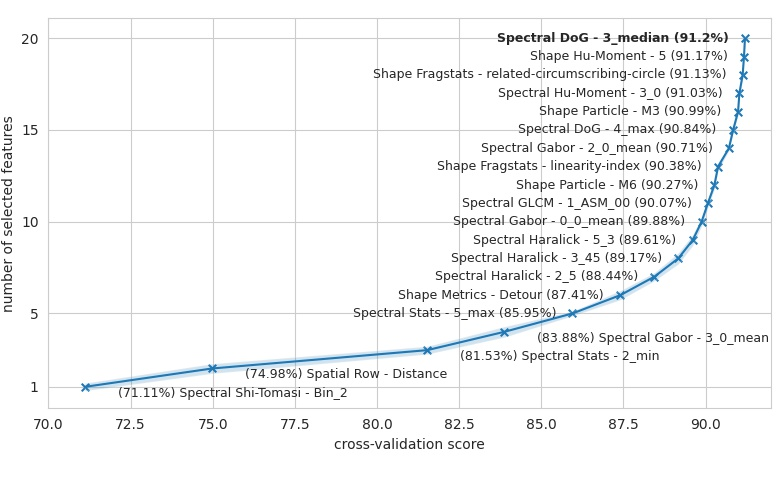
\includegraphics[width=\linewidth]{img/features/performances-plot.jpg}
        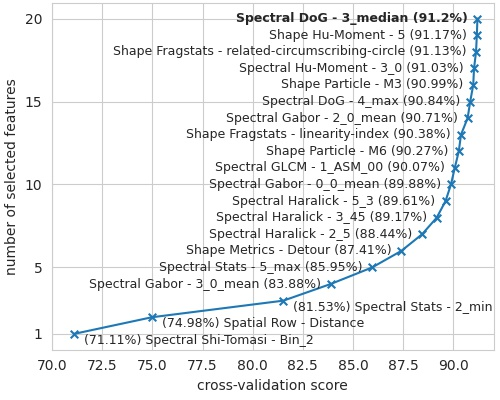
\includegraphics[]{img/features/performances-plot-small.jpg}
        \caption{Best features among all extracted feature for classification through ASHA algorithm. Best overall result is highlighted.}
        \label{fig:fv-subset-full}
    \end{figure}
    
    As shown previously (Table \ref{tab:fv-subset-spectral}), the best starting feature is the second bin of ``Spectral Shi-Tomasi'' histogram, thus it is selected firstly and its performance level is found in the first point of Figure \ref{fig:fv-subset-full} (lower-left). The second selected feature is ``Spatial Row'', it is expected that this feature should be on the top as it is a complementary with the color/texture features. At this stage, we can notice that this combination is less accurate \SI{74.98}{\percent} than two texture Haralick feature \SI{75.85}{\percent}.
    The next three features are ``Spectral Stats 2\_min'', ``Spectral Stats 5\_max'' and ``Spectral Gabor 3\_0 mean''. Which is the minimum spectral value of the underlying sub-texture of the \SI{650}{nm} spectral band for the first feature. In the same way, it is the maximum for the \SI{850}{nm} spectral band. The Gabor filter is applied on all spectral bands, the discriminating criterion is one from the \SI{450}{nm}. This leads to a performance of \SI{85.95}{\percent}. The next feature is ``Shape Metrics Detour'', with a performance of \SI{87.41}{\percent} which beats any previous classification model.
    
    To conclude on this results, the best classification model includes 1 spatial feature, 6 shape features and 13 spectral features. In the previous Figure \ref{fig:fv-subset-full}, only 20 features are shown, if more features are extracted, the performances begin to decrease (21 features = \SI{91.16}{\percent}), this means that the performance reaches a vertical asymptote. To show this a model have been learnt with all features (3545), the cross-validation score is \SI{79.97}{\percent}.
    
    \subsection{Visual results}
    Figure \ref{fig:render-roses} shows two rows with field beans plants. Weeds are located between these two rows and on each of them. Most of plant and weed leaves are correctly classified (plant leaves are colored green, and weed leaves are colored blue). However, this image suggests a problem remains for the smallest leaves that are in the center of the plant. These plants leaves, colored in red, are classified as weed leaves. This classification is induced by shape features, which are less relevant for this category of leaves than for the others. 
    
    \begin{figure}[H]
        \centering
        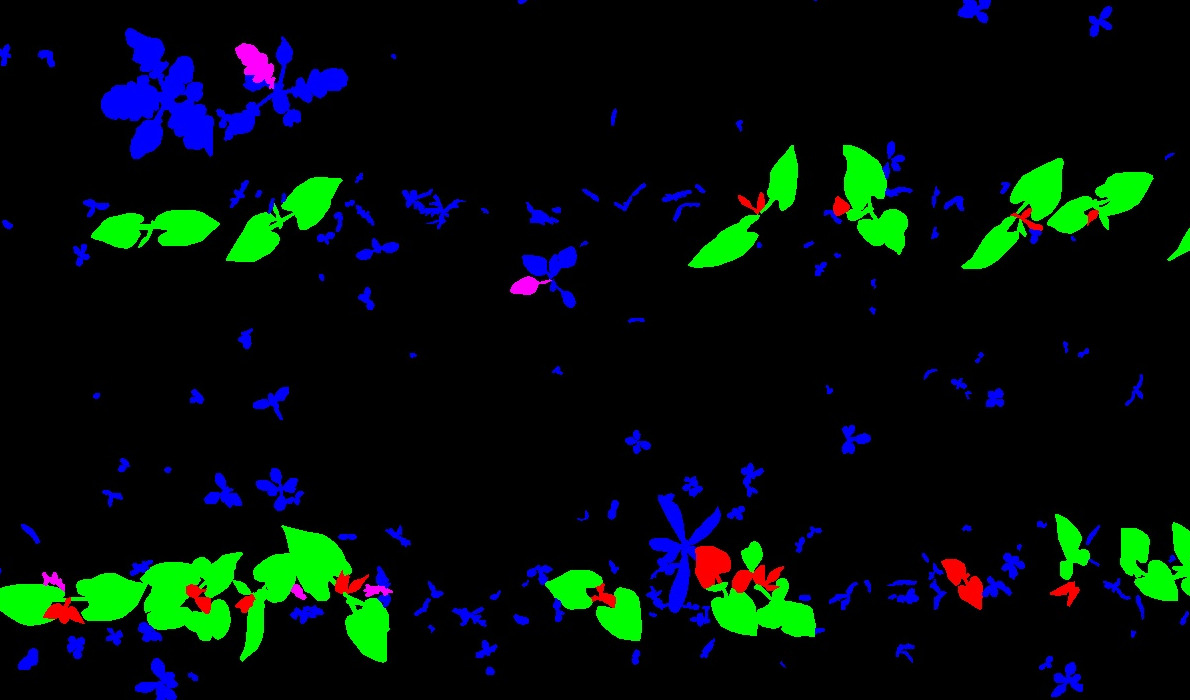
\includegraphics[width=\linewidth]{img/features/rose2.jpg}
        %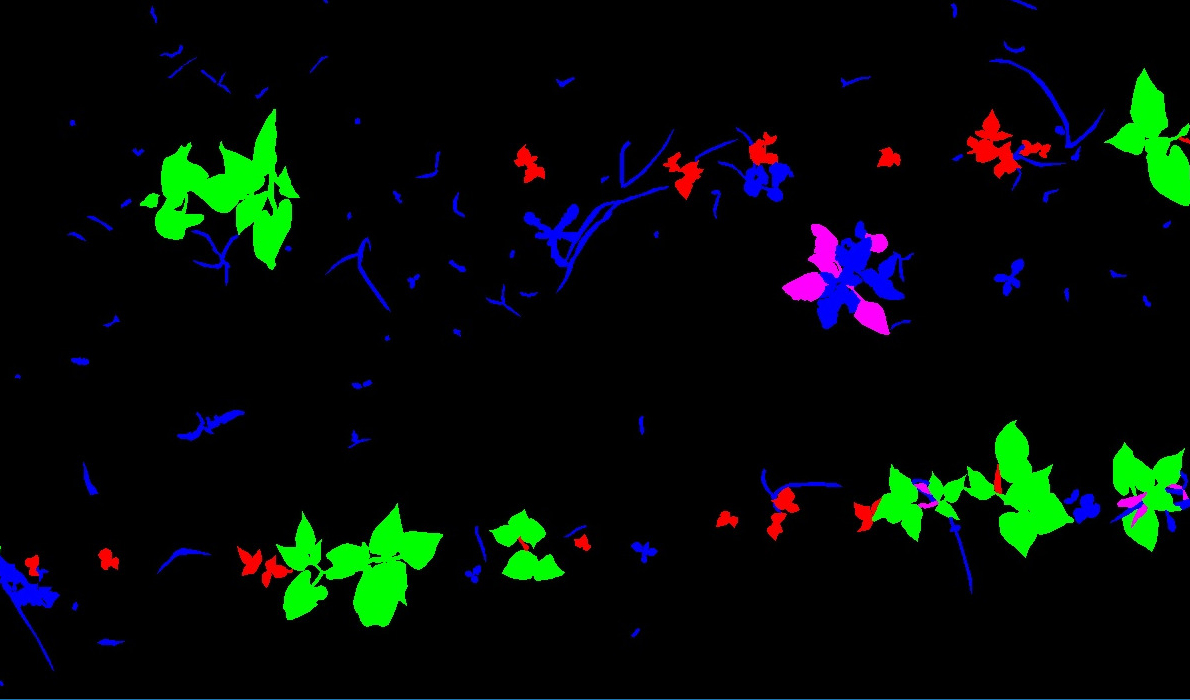
\includegraphics[width=\linewidth]{img/features/rose3.jpg}
        \caption{This figure shows the classification of leaves, from an image taken in June 2019. The blue color corresponds to well classified weeds. The green color corresponds to well classified crops. While the purple and red color correspond respectively to weeds and crops poorly classified.}
        \label{fig:render-roses}
    \end{figure}
    
    Figure \ref{fig:render-rose-2} focuses on specific parts of plant rows. Weeds on figure \ref{fig:render-rose-2}.a are mostly monocots, whereas those visible on figure \ref{fig:render-rose-2}.b are mostly dicots. These two figures illustrates the quality of classification, which is equivalent for the two weed groups. Figure \ref{fig:render-rose-2}.c presents a dense foliage, with highly developed wild mustard. On this figure, the major part of mustard leaves is correctly classified. The classification of field bean leaves depends on their visibility. Several partially occluded leaves are classified as weed leaves (in red). Conversely, figure \ref{fig:render-rose-2}.d presents sparse foliage, where many bean plants have not emerged. In that case, the small bean leaves are also classified as weed leaves.   
    
    \begin{figure}[H]
        \centering 
        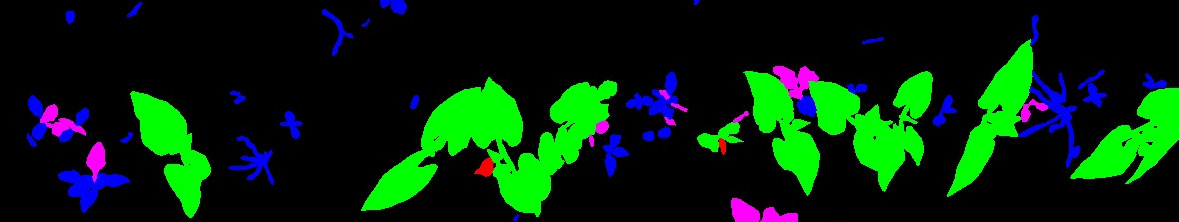
\includegraphics[width=\linewidth]{img/features/rose2-2.jpg} \\ \vspace{1em}
        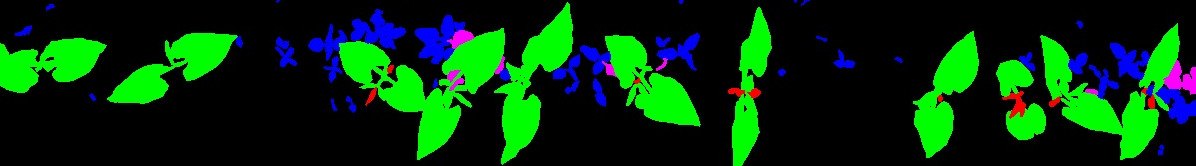
\includegraphics[width=\linewidth]{img/features/rose2-3.jpg} \\ \vspace{1em}
        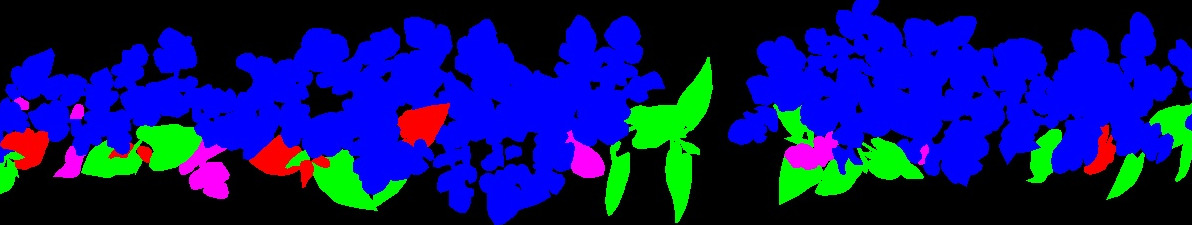
\includegraphics[width=\linewidth]{img/features/rose2-8.jpg} \\ \vspace{1em}
        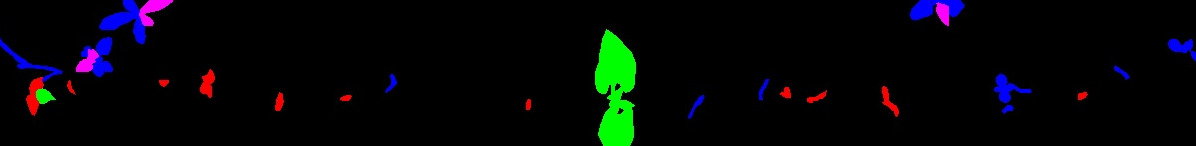
\includegraphics[width=\linewidth]{img/features/rose2-11.jpg} \\
        \caption{This figure shows the classification of leaves, from parts of four images taken in June 2019. The blue color corresponds to well classified weeds. The green color corresponds to well classified crops. While the purple and red color correspond respectively to weeds and crops poorly classified. Here we see that leaves between crop rows are correctly classified, as are monocots. On the other hand, the emerging leaves of crops and some weed type leaves of dicotyledons are incorrect.}
        \label{fig:render-rose-2}
    \end{figure}
    
    All of these images illustrate the difficulty in classifying leaves which, being in the row of crops, have particular shapes, because they are partially obscured or because they are not sufficiently developed.
    
    %!TODO table 8 -> figures
    
    %\subsection{Importance of the feature selection}
    %
    %\begin{table}
    %    \centering
    %    \rowcolors{0}{gray!10}{white}
    %    \begin{tabular}{l c}
    %        \hline
    %        \textbf{used features} & \textbf{AUC} \\
    %        \hline
    %        spatial blob        & 56.54 \\
    %        spatial corner      & 60.14 \\
    %        spatial row         & 66.93 \\
    %        \hline
    %        shape angles        & 68.38 \\
    %        shape ellipse       & 67.58 \\
    %        shape fragstats     & 71.52 \\
    %        shape metrics       & 68.94 \\
    %        shape solidity      & 63.76 \\
    %        shape particle      & 73.13 \\
    %        shape hu-moment     & 68.00 \\
    %        shape skeletonize   & 68.90 \\
    %        \hline
    %        spectral signature  & 63.65 \\
    %        spectral stats      & 74.58 \\
    %        spectral polyfit    & 70.20 \\
    %        spectral dog        & 75.76 \\
    %        spectral glcm       & 79.52 \\
    %        spectral gabor      & 74.92 \\
    %        spectral haralick   & 81.30 \\
    %        spectral hu-moment  & 71.29 \\
    %        spectral zernike    & 76.91 \\
    %        spectral lbp        & 72.61 \\
    %        spectral cslbp        & 73.03 \\
    %        spectral oclbp        & 68.12 \\
    %        spectral shi-tomasi   & 72.00 \\
    %        spectral directioanl  & 69.42 \\
    %        \hline
    %        full                & 79.97 \\
    %        \hline
    %    \end{tabular}
    %\end{table}
    
    %\subsection{Classification example}
    %\label{sec:weed-discrimination-best-all}
    
    \newpage
    \section{Conclusion}
    
    %The goal of this article was to show the potential of ASHA algorithm for big data and to present its application on a real dataset. The performance of the algorithm was quite good for a first try and the method was able to extract relevant features. The main advantage of ASHA is that it reduces the computational time and complexity by using asynchronous parallelism. The second advantage is that it can handle a hyperparameter optimization problem and can be used to optimize complex feature extraction algorithms.
    
    %\textcolor{red}{Traduction de la conclusion du chapitre 7 :}
    
    The properties we evaluated were identified from a thorough literature review. We distinguished spatial properties, based on notions of distances at the image scale, shape properties allowing to characterize the morphological features of the individuals. And, finally, properties of textures, colors and spectra were proposed to extract information related to the composition and internal structures of leaves.
    
    From this survey, it came out that some methods have parameters that influence the discrimination potential of these properties. Therefore, an algorithm was proposed to optimize these hyperparameters before the extraction and evaluation of these features. It has been shown that the optimization of these hyperparameters plays a crucial role in the performance of these criteria. For example, ``Shape Angles'' properties went from \SI{50}{\percent} to \SI{62.81}{\percent} of discrimination potential after optimization, as well as the ``Spectral DoG'' properties from \SI{46.75}{\percent} to \SI{72.39}{\percent}, etc.
    
    After the optimization of these properties, the set of properties was extracted from the dataset for evaluation. In this evaluation, it was shown the importance of selecting a smaller set of properties, the overall score is better with 20 features than all the features (3545). It is also important to notice the the contribution of each feature decreases as the number of features increases, resulting in a less interesting ``performance over computing time'' ratio. For each property type, the top 10 properties were defined. Then the top 20 among all properties combined were defined. These results show a crop/weed discrimination performance up to \SI{91}{percent} with 20 properties, while a performance of \SI{79.97}{\percent} is observed using the \SI{3545} properties. Indeed, the usual classification techniques do not seem to be able to handle large dimensions of properties. But here, the performances of classifications proposed by smaller sets are superior to the use of all the criteria. Thus, the definition of this minimal set also allows to decrease the computation time.
    
    %\subsection{Limitations}
    %
    %\textcolor{red}{Attention copier/coller vieux -> pas d'actualité}
    %
    %\paragraph{Shape}: All shape indices, based on perimeter, area, surface, area and dot relationships have %important limitations. Firstly, perimeter lengths are biased upwards in the raster images due to the stepped %line segment pattern, and the magnitude of this bias varies with the image resolution. Secondly, the %performance of the segmentation cannot guarantee a good representation of the shape, in majority of cases no %guarantee can be made to determine whether the region being segmented is a leaf, the whole plant or a group %of plants. Thus, although the patches may have very different shapes, they may have identical properties. For %this reason, it is expected that shape properties based on these criteria will be only slightly %discriminating. Alternative shape indices that are not based on perimeter-area ratios are less troubled by %these limitations. But these do not generally distinguish the morphology of patches, but rather focus on %several aspects of shape complexity. It is therefore difficult to define translation, rotation and scaling %invariant metrics, allowing the encoding of patch morphology with a good level of discrimination.
    %
    %\paragraph{Spatial}: This type of approach allows a good classification of inter-row weeds, but cannot detect %intra-row weeds. This type of property is often combined with spectral criteria and also used to set up a %semi-supervised learning where the inter-row elements are weeds, and the intra-row elements are crops and/or %indeterminate \cite{rs10050761} \textcolor{red}{attention la ref ne passe pas}.
    %
    %\paragraph{Texture} For information, the camera stores the information in u16 form (16 bit unsigned integer), %reinterpreted in float form (1 bit sign, 5 bit signifier and 10 bit exponent) with a maximum precision of %1/2047. The necessary operation transforms this float information back into u8 (8bit unsigned integer), the %precision is then 1/255. \textcolor{red}{et ? suffisant ou pas ??}
    %
    %\noindent
    %\begin{table}[H]
    %	\centering
    %    \rowcolors{0}{gray!10}{white}
    %	%\begin{adjustbox}{angle=90}
    %	\begin{tabularx}{\linewidth}{|c|X|X|}
    %		\hline
    %		\textbf{Features} & \textbf{Advantages} & \textbf{Disadvantages} \\
    %		\hline
    %		Spatial & Able to discriminate inter-row and could detect recurrent pattern in early stage & When %weed density or growth stage is advanced, these properties looses interest. \\ \hline
    %        
    %		Shape & Independent of geometric translation, scaling, or rotation and  robust to noise & Shapes are %deformed by diseases, insects eating, and man-made or mechanical damage and incomplete under overlap %and occlusion.  \\ \hline
    %        
    %		%Color &  & Crops and weeds with similar color will fail ;  \\ \hline
    %        
    %		Spectral & Robust to partial occlusion and insensitive to the adjustment of proportion, size and %position & Spectral features vary in different growth stages of plants, are easily affected by %environmental factors. Leaf lesions and plant seasonality also change spectral properties. \\ \hline
    %        
    %        Texture & Has high accuracy, strong adaptability and robustness & Takes a long time and does not meet %the real-time processing requirements. \\ 
    %		\hline
    %	\end{tabularx}
    %	%\end{adjustbox}
    %	\caption{Comparison of the advantages and disadvantages of four common features.}
    %\end{table}
    
    %The results show that for each feature type, there is a good trade-off between the number of extracted features and their performance on the classification task. This suggests that we can use only a few features of each type to perform a good classification task. However, when we consider all features, we need to use more features to obtain a good classification performance. This can be explained by the fact that some categories are more discriminative than others and that some feature types are more discriminative than others.
    
    \newpage
    \section{Further research}
    
    Today, deep learning may be the only competitive alternative that could improve the results of each feature type. Following the approach that has been undertaken in a previous article \cite{Vayssade2021}, an alternative based on function approximators is possible. We could then define the best shape properties from a fixed representation of the contour. The same is true for texture and spatial properties. In reality, a UNet model already synthesizes the set of texture, color, spectrum and a kind of shape features if used in this crop/weed discrimination framework. Moreover, the performance of the extraction of these features does not allow a real time use, which reinforces the need to study deep learning.
    
    In this study, feature selection is only based on classification performances of features. Computation speed is neither estimated nor taken into account. However, depending on the application, a compromise between computation speed and classification performance could be used. The selection of the best features for real-time weed detection and elimination is of particular interest. Figure \ref{fig:fv-subset-full} shows that the major classification improvement comes from the 10 first features (from \SI{71} to \SI{90}{\percent}), the next 10 features improve the classification result of a bit more than \SI{1}{\percent}. This observation shows that a study focused on performance over computing time should be relevant. This is also a key step in developing on-board weed control systems in autonomous vehicles where computing power can be restricted and time matters the most. 
    
    Considering precision farming applications, this approach could be replicated to select the best features for a specific set of crop(s) and weeds. The objective could change from an application to another and should be linked to the classification accuracy requirements and the time available. A real-time application may focus on computing time with less consideration for classification performance. A UAV approach may allow more computing time as the result is already delayed from the acquisition. In both case, the image resolution may be an important setting: too high and the computing time may be too important, too low and the classification performance may drop too much. This resolution may also impact the feature contribution to the overall classification with spectral or shape feature requiring highest resolution than spatial features.
    
    
    % Conlusion générale de la thèse
    
    % Une performance de classification de \SI{91}{\percent} a été démontrée. Nous rappelons que notre étude est à l'échelle de la feuille, ce qui est une première dans ce domaine, ainsi qu'en condition terrain. Il n'existe donc pas de points de comparaison dans la littérature. Nous pouvons cependant noter qu'à l'échelle de la plante dans différentes conditions d'acquisition, l'état de l'art \cite{Ahmed2016} donne des performances entre \SI{77}{\percent} et \SI{97}{\percent} de discrimination cultures/adventices. Ce qui place favorablement nos résultats et offre ainsi des perspectives intéressantes.
    
    %\textcolor{red}{add figures d'exemples de résultat de classif dans R et D et voir si on peut discuter des limites, par exemple feuilles dans le rang? feuilles partielles? ...}
    
    %\textcolor{red}{rmqGJ: ok avec le texte qui a plus sa place dans la section R&D, je l'ai déplacé et ai ajouté la subsection "Visual results"}
    
    \newpage
    \section*{Supplementary materials}
    
    \null
    \vfill
    \begin{table}[H]
        \centering
        \rowcolors{0}{gray!10}{white}
        %\begin{adjustbox}{angle=270}
        \begin{tabular}{|c|c|c|c|}
            \hline
            \textbf{Type} & \textbf{Name}		& \textbf{FV} & \textbf{HP} \\
            \hline
            Spatial & Borner  		&   1 & 4 \\
            Spatial & Row     		&   1 & 6 \\
            Spatial & Blob    		&   1 & 4 \\
            \hline
            \textbf{type} & \textbf{name}		& \textbf{FV} & \textbf{HP} \\
            \hline
            Shape & Angles			&   9 & 5 \\
            Shape & Ellipse	 		&  11 & -- \\
            Shape & Fragstat		&   6 & -- \\
            Shape & metrics			&   8 & -- \\
            Shape & Solidity		&   1 & -- \\
            Shape & Particle		&  18 & -- \\
            Shape & Hu Moment		&   7 & -- \\
            Shape & Skeletonize		&   4 & -- \\
            &&& \\
            &&& \\
            \hline
        \end{tabular}
        \begin{tabular}{|c|c|c|c|}
            \hline
            \textbf{Type} & \textbf{Name}		& \textbf{FV} & \textbf{HP} \\
            \hline
            Spectral & Sig			&  16 & -- \\
            Spectral & Stats		&  72 & -- \\
            Spectral & polyfit		&  58 & 1 \\
            
            Spectral & DoG			&   72 & 2 \\
            Spectral & HOG			&   72 & 1 \\
            Spectral & Gabor		&  288 & 4 \\
            Spectral & Haralick		&  416 & 1 \\
            Spectral & GLCM			&   80 & 2 \\
            Spectral & Hu Moment	&   56 & -- \\
            Spectral & Zernike		&   32 & 2 \\
            Spectral & LBP			& 2056 & 1 \\
            Spectral & CSLBP		&  144 & 1 \\
            Spectral & OCLBP		&   34 & -- \\
            Spectral & Shi-Tomasi	&    8 & 1 \\
            %spectral & non max		&   -- & 1 \\
            \hline
        \end{tabular}
        %\end{adjustbox}
        \caption{Number of features after hyperparameter optimization (FV) and number of hyperparameters (HP) per feature extraction methods}
        \label{tab:optimized_features}
    \end{table}
    \vfill
    \begin{table}[H]
        \rowcolors{0}{gray!10}{white}
        \begin{tabularx}{\linewidth}{|l|X|}
            \hline
            Shape Angles & bins\_8, bins\_12, bins\_13, bins\_14, bins\_15, bins\_16, bins\_17, bins\_18, bins\_19, bins\_20 \\ \hline
            
            Shape Ellipse & center-distance, minor-axis, angle, eccentricity\_1, eccentricity\_2, eccentricity\_3, eccentricity\_angle, focal-distance, directrice, det \\ \hline
            
            Shape Fragstats & perimeter-area-ratio, shape-index, fractal-dimension\_index, linearity-index, related-circumscribing-circle, perimeter-area-fractal-dimension \\ \hline
            
            Shape Hu-Moment & 0, 1, 2, 3, 4, 5, 6 \\ \hline
            
            Shape Metrics & proximity, spin, area-exchange, perim-index, depth, dispersion, girth, detour \\ \hline
            
            Shape Particle & inv-area, inv-perimeter, m2, m3, m4, m6, m8, aspect-ratio, roundness, convexity \\ \hline
            
            Shape Skeletonize & pixel-count, end-point, itersection, branch-count \\ \hline
        \end{tabularx}
        \caption{Top features for each shape types}
        \label{tab:feature-name-shape}
    \end{table}
    \vfill
    \null
    
    \newpage
    
    \null
    \vfill
    \begin{table}[H]
        \rowcolors{0}{gray!10}{white}
        \begin{tabularx}{\linewidth}{|l|X|}
            \hline
            Spectral CSLBP & bins\_0\_21, bins\_1\_10, bins\_1\_18, bins\_1\_19, bins\_1\_20, bins\_1\_21, bins\_2\_10, bins\_2\_18, bins\_2\_20, bins\_4\_21 \\ \hline
            
            %Spectral Directional & bins\_0, bins\_1, bins\_2, bins\_3, bins\_4, bins\_5, bins\_6, bins\_7 \\ \hline
            
            Spectral DoG & 0\_median, 2\_min, 2\_median, 3\_max, 3\_median, 3\_entropy, 4\_max, 5\_max, 5\_mean, std\_max \\ \hline
            
            Spectral Gabor & 0\_0\_median, 1\_0\_mean, 2\_0\_max, 2\_0\_mean, 3\_0\_min, 3\_158\_entropy, 4\_0\_min, 5\_0\_min, std\_158\_mean, ndvi\_0\_min \\ \hline
            
            Spectral HOG & 0\_bins\_70, 1\_bins\_70, 1\_bins\_130, 2\_bins\_70, 3\_bins\_30, 5\_bins\_110, std\_bins\_30, std\_bins\_70, std\_bins\_150, ndvi\_bins\_150 \\ \hline
            
            Spectral GLCM & 0\_ASM\_00, 1\_contrast\_90, 3\_correlation\_90, 3\_ASM\_90, 4\_contrast\_90, 4\_homogeneity\_00, 5\_contrast\_90, std\_contrast\_90, std\_correlation\_90, ndvi\_homogeneity\_90 \\ \hline
            
            Spectral Haralick & 1\_17, 1\_31, 2\_24, 2\_31, 3\_32, 4\_32, 5\_3, 5\_51, std\_29, std\_44 \\ \hline
            
            Spectral Hu-Moment & 0\_0, 1\_1, 2\_1, 3\_0, 3\_2, 4\_0, 5\_0, 5\_4, std\_3, ndvi\_3 \\ \hline
            
            Spectral LBP & bins\_0\_64, bins\_0\_209, bins\_1\_129, bins\_2\_129, bins\_2\_209, bins\_3\_129, bins\_4\_209, bins\_4\_250, bins\_5\_129, bins\_std\_129 \\ \hline
            
            Spectral OCLBP & bins\_0, bins\_1, bins\_2, bins\_3, bins\_4, bins\_9, bins\_20, bins\_26, bins\_32, bins\_33 \\ \hline
            
            Spectral Polyfit & 1\_2, 1\_6, 2\_6, 3\_1, 3\_6, 4\_4, 5\_3, 5\_4, std\_5, ndvi\_0 \\ \hline
            
            Spectral Shi-tomasi & bins\_0, bins\_1, bins\_2, bins\_3, bins\_4, bins\_6, bins\_7, bins\_9, bins\_11, bins\_13 \\ \hline
            
            Spectral Signature & shape\_0, shape\_1, shape\_2, shape\_3, shape\_4, shape\_5, shape\_ndvi, window\_0, window\_std, window\_ndvi \\ \hline
            
            Spectral Stats & 0\_min, 1\_std, 2\_min, 2\_median, 3\_max, 3\_median, 4\_std, 4\_entropy, 5\_max, ndvi\_max \\ \hline
            
            Spectral Zernike & 0\_A, 1\_Zr, 1\_A, 2\_Zr, 3\_A, 4\_A, 5\_A, std\_A, std\_Phi, ndvi\_A \\ \hline
        \end{tabularx}
        \caption{Top 10 for each spectral types}
        \label{tab:feature-name-spectral}
    \end{table}
    \vfill
    \null
    
    %\begin{table}[H]
    %    \rowcolors{0}{gray!10}{white}
    %    \begin{tabularx}{\linewidth}{|l|X|}
    %        \hline
    %        Spatial Row & distance \\\hline
    %        Shape Dragstats & linearity-index, related-circumscribing-circle \\\hline
    %        Shape Metrics & detour \\\hline
    %        Shape Particle & m3, m6 \\\hline
    %        Shape Hu-Moment & 5 \\\hline
    %        Spectral Stats & 0\_min, 2\_min, 5\_max \\\hline
    %        Spectral DoG & 3\_median, 4\_max \\\hline
    %        Spectral GLCM & 1\_ASM\_00 \\\hline
    %        Spectral Gabor & 0\_0\_mean, 2\_0\_mean, 3\_0\_mean \\\hline
    %        Spectral Haralick & 2\_5, 3\_45, 5\_3\\\hline
    %        Spectral Hu-Moment & 3\_0 \\ \hline
    %        %spatial\_row & distance \\ \hline
    %        %shape\_ellipse & eccentricity\_3 \\ \hline
    %        %shape\_fragstats & fractal-dimension\_index, related-circumscribing-circle \\ \hline
    %        %shape\_metrics & dispersion \\ \hline
    %        %shape\_particle & m2 \\ \hline
    %        %shape\_hu-moment & 1, 3 \\ \hline
    %        %spectral\_stats & 1\_kurtosis \\ \hline
    %        %spectral\_glcm & 0\_ASM\_90, 1\_dissimilarity\_90, 3\_ASM\_00 \\ \hline
    %        %spectral\_gabor & std\_0\_mean,  ndvi\_45\_mean, ndvi\_90\_mean \\ \hline
    %        %spectral\_haralick & 1\_38, 3\_16, 5\_45, std\_38 \\ \hline
    %        %spectral\_hu-moment & 2\_6 \\ \hline
    %    \end{tabularx}
    %    \caption{Top 20 features among all features}
    %    \label{tab:feature-name-mixed}
    %\end{table}
    
    %\begin{table}[H]
    %    \centering
    %    \rowcolors{0}{gray!10}{white}
    %    \begin{tabular}{|c|l|l||c|l|l|}
    %        \hline
    %        \textbf{ID} & \textbf{Type} & \textbf{Name} &
    %        \textbf{ID} & \textbf{Type} & \textbf{Name} \\
    %        \hline
    %        1 & Spectral Shi-Tomasi & Bin\_2        &
    %        2 & Spatial Row         & Distance      \\
    %        3 & Spectral Stats      & 2\_min        &
    %        4 & Spectral Gabor      & 3\_0\_mean    \\
    %        5 & Spectral Stats      & 5\_max        &
    %        6 & Shape Metrics       & Detour        \\
    %        7 & Spectral Haralick   & 2\_5          &
    %        8 & Spectral Haralick   & 3\_45         \\
    %        9 & Spectral Haralick   & 5\_3          &
    %       10 & Spectral Gabor      & 0\_0\_mean    \\
    %       
    %       11 & Spectral GLCM       & 1\_ASM\_00    &
    %       12 & Shape Particle      & M6            \\
    %       13 & Shape Fragstats     & linearity-index &
    %       14 & Spectral Gabor      & 2\_0\_mean    \\
    %       15 & Spectral DoG        & 4\_max        &
    %       16 & Shape Particle      & M3            \\
    %       17 & Spectral Hu-Moment  & 3\_0          &
    %       18 & Shape Fragstats     & related-circumscribing-circle \\
    %       19 & Shape Hu-Moment     & 5             &
    %       20 & Spectral DoG        & 3\_median     \\
    %        \hline
    %    \end{tabular}
    %    \caption{Top 20 features among all features}
    %    \label{tab:feature-name-mixed}
    %\end{table}
    
    %\begin{figure}[H]
    %    \centering \vspace{2pt}
    %    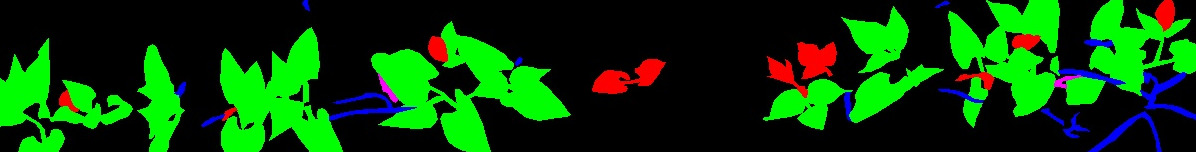
\includegraphics[width=\linewidth]{img/features/rose3-1.jpg} \vfill
    %   %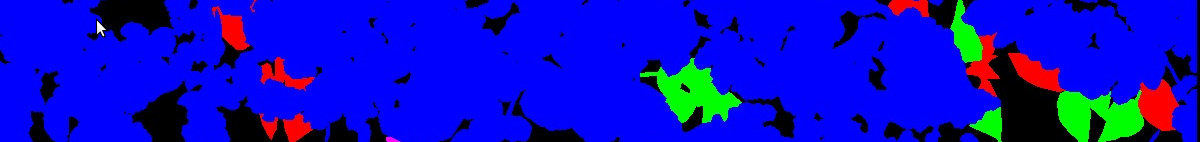
\includegraphics[width=\linewidth]{img/features/rose3-2.jpg} \vfill
    %    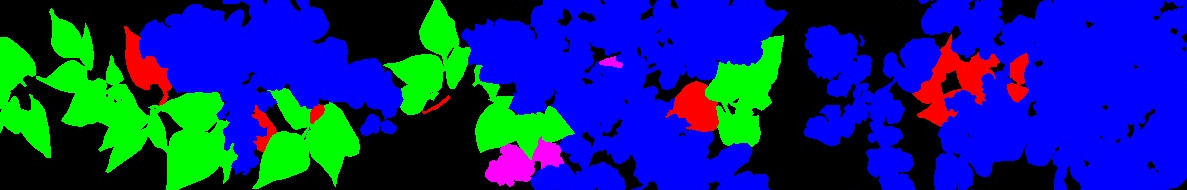
\includegraphics[width=\linewidth]{img/features/rose3-3.jpg} \vfill
    %    %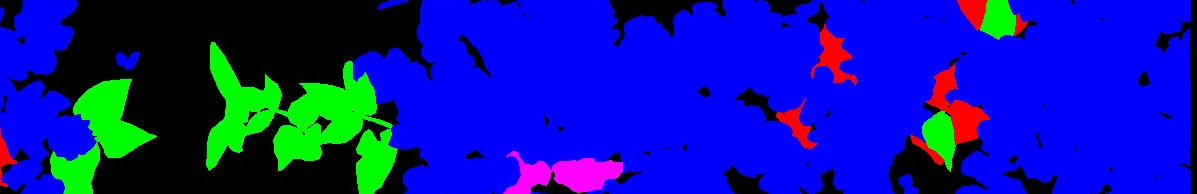
\includegraphics[width=\linewidth]{img/features/rose3-4.jpg} \vfill
    %    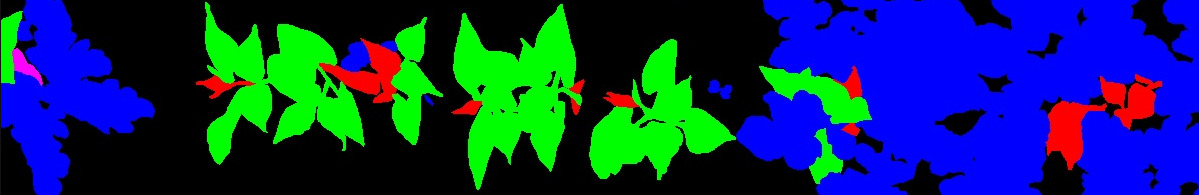
\includegraphics[width=\linewidth]{img/features/rose3-5.jpg} \vfill
    %    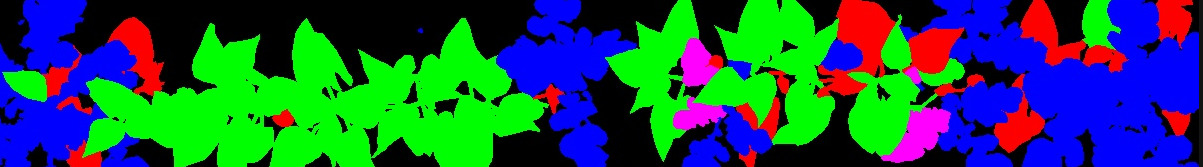
\includegraphics[width=\linewidth]{img/features/rose3-6.jpg} \vfill
    %    %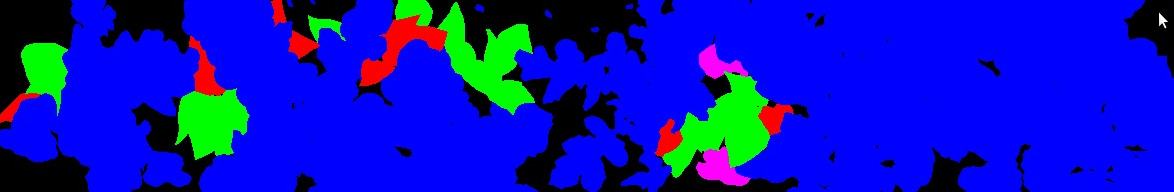
\includegraphics[width=\linewidth]{img/features/rose3-7.jpg} \vfill
    %    %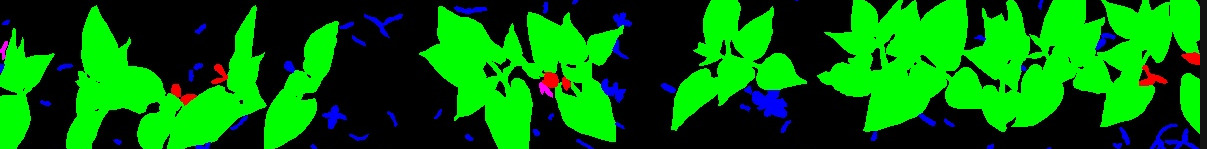
\includegraphics[width=\linewidth]{img/features/rose3-8.jpg}
    %    \caption{Rose 3}
    %    \label{fig:render-rose-3}
    %\end{figure}
    
    \section*{Funds \& Conflicts of Interest}  Funding was received from the European Union’s Horizon 2020 research and innovation program under grant agreement No 727321 (project acronym, IWMPRAISE). It was also funded by the French National Research Agency Challenge RoSE [grant agreement ID: ANR-17-ROSE-0002] (project acronym: ROSEAU). In addition, a collaboration with SITIA company is existing. The authors declare that they have no known competing financial interests or personal relationships that could have appeared to influence the work reported in this paper
    \vfill
    
	\newpage
	\section{Conclusion de chapitre}
    
    %V.1
    %L'extraction de propriété pour la classification d'objet est une technique standard. Dans le cadre de cette thèse, nous avons voulu définir les meilleurs d'entre eux pour la discrimination cultures/adventices. Car il n'existe pas d'études les définissants clairement (souvent un petit ensemble de propriétés, dans des conditions spécifiques, \dots). De plus, dans cette thèse, il a été défini une échelle de segmentation plus fine que la plante : celle de la feuille.
    
    %V.2
    L'un des buts de cette thèse était de définir les meilleures propriétés pour la discrimination culture/adventices. Comme il n'existe pas d'études les définissant clairement (souvent, un petit ensemble de propriétés, dans des conditions spécifiques, est utilisé.), nous avons mené nos propres recherches pour identifier les méthodes les plus prometteuses. De plus, une échelle de segmentation plus fine que celle de la plante a été définie, celle de la feuille. Ce faisant, nous espérons fournir une compréhension plus détaillée de la manière dont ces propriétés peuvent être utilisées à des fins de classification cultures/adventices.
    
    %Ainsi l'article qui a été présenté ci-avant propose une méthodologie complète sur ce sujet.
    Pour combler cette lacune, nous avons recensé les méthodes existantes et identifiées les propriétés les plus prometteuses pour la discrimination cultures/adventices à l'échelle de la feuille. On y distingue les propriétés spatiales, reposant sur des notions de distances à l'échelle de l'image, et les propriétés de forme permettant de caractériser les traits morphologiques des individus. Des propriétés de texture, de couleur et de spectre ont également été proposées pour extraire des informations liées à la composition et aux structures internes des feuilles (veines, épiderme, \dots).
    
    À partir de ce recensement, nous avons vu que certaines méthodes permettant d'extraire des propriétés comportaient des paramètres. Ces paramètres influencent le potentiel de discrimination des propriétés extraites. C'est pourquoi un algorithme a été proposé pour optimiser ces paramètres avant l'extraction et l'exploitation des propriétés concernées. Il a été montré que l'optimisation de ces hyperparamètres jouait un rôle crucial. Par exemple, les propriétés du type ShapeAngles passent de \SI{50}{\percent} a \SI{62.81}{\percent} de potentiel de discrimination après optimisation, de même que les propriétés SpectralDoG passent de \SI{46.75}{\percent} à \SI{72.39}{\percent}, etc.
    
    %Après l'optimisation de ces propriétés, l'ensemble de données a été évalué pour déterminer l'importance de la sélection d'un ensemble plus restreint de propriétés. Les 10 meilleures propriétés ont été définies pour chaque type de propriété, puis les 20 meilleures propriétés parmi tous les types combinées de propriétés. Ces résultats ont montré qu'une performance de discrimination culture/adventice jusqu'à 91% est possible en utilisant un ensemble de 20 propriétés, alors qu'une performance de 79.97% est observée en utilisant les 3545 propriétés. Cela démontre que la sélection d'un ensemble plus restreint de propriétés permet d'obtenir des performances de classification supérieures à l'utilisation de tous les critères. De plus, cette sélection permet également de réduire le temps de calcul.
    
    Après cette phase d'optimisation, toutes les propriétés ont été extraites à partir du jeu de données pour évaluation. Au cours de cette évaluation, il a été montré l'importance de la sélection d'un ensemble plus petit de propriétés. Les 10 meilleures ont été sélectionnées pour chaque type de propriété, puis les 20 meilleures parmi toutes les propriétés combinées. Les résultats montrent une performance de discrimination culture/adventices à hauteur de \SI{91}{\percent} avec 20 propriétés, tandis qu'une performance de \SI{79.97}{\percent} est observée en utilisant l'ensemble des \SI{3545} propriétés. En effet, les techniques de classification usuelles ne semblent pas être capables de gérer de grands ensembles de propriétés. Par conséquent, il est important de définir un ensemble minimal de critères qui permette de diminuer le temps de calcul tout en maximisant les performances de classification.
    % Mais ici, les performances des classifications proposées par des ensembles plus petits sont supérieures à l'utilisation de tous les critères. Ainsi, la définition de cet ensemble minimal permet également de diminuer le temps de calcul.
    
    %version courte ... à enlever ?
    % JNP : à mon avis oui
    En conclusion, une étude a été réalisée pour déterminer quelles propriétés sont les plus importantes pour la tâche de discrimination cultures/adventices, puis elles ont été optimisées pour obtenir les meilleurs résultats. Un algorithme a été utilisé pour trouver la meilleure façon d'utiliser ces propriétés pour la classification. Au final, il a été constaté que l'utilisation d'un ensemble plus restreint de propriétés, de différents types, donne les meilleurs résultats.
	
\end{document}

